\documentclass[xcolor={dvipsnames}]{beamer}

\usepackage{amsmath}
\usepackage{amsthm}
\usepackage[T1]{fontenc}
\usepackage[utf8]{inputenc}
\usepackage{MnSymbol}
\usepackage{stmaryrd}
\usepackage{upquote}
\usepackage{bussproofs, semantic, framed}
\usepackage{array}
\usepackage{hyperref}

\usepackage{graphicx}
\usepackage{cellspace}
\setlength\cellspacetoplimit{4pt}
\setlength\cellspacebottomlimit{4pt}
% for showing frames while development
%\usepackage{showframe}
\usepackage{caption, subcaption, wrapfig}
\usepackage{textcomp, scrextend}
%\usepackage{xcolor}
\usepackage{babel}
\usepackage{url}
\usepackage{setspace}
\usepackage{esint}
\usepackage{natbib}

% \usepackage{minted}
\definecolor{ltblue}{rgb}{0,0.4,0.4}
\definecolor{dkblue}{rgb}{0,0.1,0.6}
\definecolor{dkgreen}{rgb}{0,0.4,0}
\definecolor{dkviolet}{rgb}{0.3,0,0.5}
\definecolor{dkred}{rgb}{0.5,0,0}
\definecolor{battleshipgrey}{rgb}{0.52, 0.52, 0.51}

\usepackage{listings}

\usepackage{haskell}
\usepackage{cmll}
\usepackage{pdflscape}

\usepackage{tikz}
\usepackage{tikz-qtree}
%\usetikzlibrary{arrows.meta}

\usepackage{parskip}
\usepackage{xspace}

\usepackage[style=british]{csquotes}

\def\signed #1{{\leavevmode\unskip\nobreak\hfil\penalty50\hskip2em
  \hbox{}\nobreak\hfil--- #1%
  \parfillskip=0pt \finalhyphendemerits=0 \endgraf}}

\newsavebox\mybox
\newenvironment{aquote}[1]
  {\savebox\mybox{#1}\begin{quote}}
  {\signed{\usebox\mybox}\end{quote}}


\usepackage[capitalize, nameinlink]{cleveref}
\crefformat{section}{\S#2#1#3} % see manual of cleveref, section 8.2.1
\crefformat{subsection}{\S#2#1#3}
\crefformat{subsubsection}{\S#2#1#3}


\newcommand\fnurl[2]{%
  \href{#2}{#1}\footnote{\url{#2}}%
}
\mode<presentation>{\usetheme{Madrid}}


\newcommand{\tightoverset}[2]{%
  \mathop{#2}\limits^{\vbox to -.5ex{\kern-0.75ex\hbox{$#1$}\vss}}}

\newcommand{\BI}{\textbf{\em BI}\xspace}
\newcommand{\HM}{\textbf{\em HM}\xspace}
\newcommand\sepimp{\mathrel{-\mkern-6mu*}}
\newcommand\shimp{\twoheadrightarrow}

\newcommand{\M}{\mathcal{M}}
\newcommand{\W}{\mathcal{W}}
\newcommand{\Unf}{\mathcal{U}}
\newcommand{\Fun}[1]{\texttt{Fun}\ #1}
\newcommand{\SeFun}[1]{\texttt{SeFun}\ #1}
\newcommand{\ShFun}[1]{\texttt{ShFun}\ #1}
\newcommand{\Un}[1]{\texttt{Un}\ #1}
\newcommand{\vdashs}{\vdash^s}
\newcommand{\Gen}[1]{\texttt{Gen}(#1)}
\newcommand{\Let}[3]{\texttt{let}\ #1 = #2\ \texttt{in}\ #3}
\newcommand{\Case}[2]{\texttt{case}\ #1\ \texttt{of}\ #2}
\newcommand{\Fst}[1]{\texttt{fst}\ #1}
\newcommand{\Snd}[1]{\texttt{snd}\ #1}
\newcommand{\Inr}[1]{\texttt{inr}\ #1}
\newcommand{\Inl}[1]{\texttt{inl}\ #1}
\newcommand{\Pair}[1]{\langle #1 \rangle}
\newcommand{\qub}{QuB\xspace}

\usepackage{halloweenmath}
\usepackage[normalem]{ulem}

\title{\qub{}}
\subtitle{A Resource Aware Functional Programming Language}
\author{Apoorv Ingle}
\date{}
\institute[KU]{The University of Kansas}
% disable useless navigation symbols
\setbeamertemplate{navigation symbols}{}

% disable the section information
% \setbeamertemplate{headline}{}

\begin{document}
\frame\titlepage

\begin{frame}
  \frametitle{Table of Contents}
  \tableofcontents
\end{frame}

% Introduction and motivation
% 5 mins
\section{Introduction and Motivation}\label{sec:introduction}
% (5 mins)

\begin{frame}[c]
  \frametitle{Introduction and Motivation}
  {\large
    \begin{center}
      Hard problems in programming

      {\LARGE \color{red}Naming variables}
    \end{center}
    }
\end{frame}

\begin{frame}
  \frametitle{Introduction and Motivation}
  \begin{center}
    {\large Hard problems in programming}

    {\LARGE \color{red}Resource management}
    \\{\normalsize  in evolving production code}

    {\normalsize Resources: Files, database connections, shared mutable state}
\end{center}
\end{frame}

\begin{frame}[fragile, c]
  \frametitle{Resource Management: File Handling}
  \begin{center}
    \begin{itemize}
    \item Modified File Handling API in Haskell
    \end{itemize}
    \begin{tabular}[h]{c}
      \begin{haskell}

     openFile   :: FilePath   -> IO FileHandle

     closeFile  :: FileHandle -> IO ()

     readLine   :: FileHandle -> IO (String, FileHandle)

     writeLine  :: FileHandle -> String
                              -> IO FileHandle


     upper      :: String     -> String

     ($\gg\!=$) :: IO a -> (a -> IO b) -> IO b
      \end{haskell}
    \end{tabular}
\end{center}
\end{frame}

\begin{frame}[fragile,c]
  \frametitle{Resource Management: File Handling}
  \begin{center}
    \begin{itemize}
    \item File Handling in Haskell
    \end{itemize}
    \begin{tabular}[h]{c}
      \begin{haskell}
        do f  <- openFile "sample.txt"
           (s, f)  <- readLine f
           let c = upper s
           f <- writeLine f c
                  .
                  .
                  .
           () <- closeFile f
      \end{haskell}
    \end{tabular}
  \end{center}
\end{frame}

\begin{frame}[fragile, c]
  \frametitle{Resource Management: File Handling}
  \begin{center}
    \begin{itemize}
    \item File Handling in Haskell Gone Wrong (Part I)
    \end{itemize}
    \begin{tabular}[h]{c}
    \begin{haskell}
      do f  <- openFile "sample.txt"
         (s, f)  <- readLine f
         let c = upper s
         f <- writeLine f c
              .
              .
              .
         () <- closeFile f
              .
              .
              .
         () <- closeFile f
         return c
    \end{haskell}
    \end{tabular}
  \end{center}
\end{frame}

\begin{frame}[fragile, c]
  \frametitle{Resource Management: File Handling}
  \begin{center}
    \begin{itemize}
    \item File Handling in Haskell Gone Wrong (Part I)
    \end{itemize}
    \begin{tabular}[h]{c}
    \begin{haskell}
      do f  <- openFile "sample.txt"
         (s, f)  <- readLine f
         let c = upper s
         f <- writeLine f c
              .
              .
              .
        @() <- closeFile f@
              .
              .
              .
        @() <- closeFile f@
         return c
    \end{haskell}
    \end{tabular}
    \begin{itemize}
    \item File is closed twice: Run time crash
    \end{itemize}
  \end{center}
\end{frame}

\begin{frame}[fragile, c]
  \frametitle{Resource Management: File Handling}
  \begin{center}

  \begin{itemize}
  \item File Handling in Haskell Gone Wrong (Part II)
  \end{itemize}
  \begin{tabular}[h]{c}
    \begin{haskell}
    do f  <- openFile "sample.txt"
       (s, f)  <- readLine f
       let c = upper s
       f <- writeLine f c
           .
           .
           .
       return c
     \end{haskell}
  \end{tabular}

\end{center}
\end{frame}

\begin{frame}[fragile, c]
  \frametitle{Resource Management: File Handling}
  \begin{center}

  \begin{itemize}
  \item File Handling in Haskell Gone Wrong (Part II)
  \end{itemize}
  \begin{tabular}[h]{c}
    \begin{haskell}
    do f  <- openFile "sample.txt"
       (s, f)  <- readLine f
       let c = upper s
       f <- writeLine f c
           .
           .
           .
       return c {- File not closed!! -}
     \end{haskell}
  \end{tabular}
  \begin{itemize}
  \item File not closed: Memory leak
  \end{itemize}
  \end{center}
\end{frame}

\begin{frame}[fragile, c]
  \frametitle{Resource Management: Exception Handling}
  \begin{center}
    \begin{itemize}
    \item \texttt{MonadError}\footnote[frame]{\fullcite{liang_monad_1995}}  type class in Haskell
      \begin{tabular}[c]{c}
        \begin{haskell}
      class Monad m => MonadError e m | m -> e where
          throwError :: e -> m a
          catchError :: m a -> (e -> m a) -> m a
        \end{haskell}
      \end{tabular}

    \item\texttt{MonadError} instance with \texttt{IO} and \texttt{Exception}
      \begin{tabular}[c]{c}
        \begin{haskell}
          throwError :: Exception -> IO a
          catchError :: IO a -> (Exception -> IO a) -> IO a
        \end{haskell}
      \end{tabular}

    \item \texttt{throwError} start exception processing
    \item \texttt{catchError} exception handler
    \end{itemize}
  \end{center}
\end{frame}

\begin{frame}[fragile, c]
  \frametitle{Resource Management: Exception Handling}
  \begin{center}

  \begin{itemize}
  \item Using \texttt{MonadError} in Haskell
  \end{itemize}
  \begin{tabular}[h]{c}
    \begin{haskell}
  (do f <- openFile "sample.txt"
     @(s, f)  <- readLine f@         {- Exception raised here -}
      let c = upper s
      () <- closeFile f
      return \dollar Right c)
          `catchError` (\_ ->
                 return \dollar Left "Error in reading file")
     \end{haskell}
  \end{tabular}
  \begin{itemize}
  \item Exception may cause memory leak
  \end{itemize}
  \end{center}
\end{frame}

\begin{frame}[c]
  \frametitle{Introduction and Motivation}
  \begin{center}
    \uncover<+-> {\LARGE
      \begin{aquote}{R. Milner}
        Well typed programs do not go wrong.
      \end{aquote}
    }
    \vspace{2cm}
    % \begin{description}
    % \item<2-> \qquad \qquad {\color{red}Can we do better?}
    % \end{description}
    \uncover<+-> {\LARGE
      \begin{aquote}{Coldplay}
        \sout{Lights}{\color{red} Types} will guide you home$\dots$
      \end{aquote}
    }
  \end{center}
\end{frame}

\begin{frame}
  \frametitle{Contributions}

  \begin{itemize}

  \item {\color{red}Language design}
    \begin{itemize}
    \item {\color{red}Resources are ``first class citizens''}
    \item {\color{red}Resources(variables) can be in sharing or separate}
    \end{itemize}

  \item {\color{red}\qub{} is logic of \BI on steroids}
    \begin{itemize}
    \item {\color{red}Typing Environments as graphs}
    \end{itemize}
  \item {\color{red}Working examples}
  \item Formalizing and proving important properties of \qub{}
    \begin{itemize}
    \item Type system
    \item Syntax directed type system (sound and complete)
    \item Type inference algorithm $\M$ (sound)
    \end{itemize}

  \end{itemize}

\end{frame}


%%% Local Variables:
%%% mode: latex
%%% TeX-master: "defense-slides"
%%% End:


% Background work
% 8 mins
\section{Background Work}\label{sec:background}
% (10 mins)

\begin{frame}[fragile, c]
    \frametitle{Background Work: STLC and \HM{} type system}
    \begin{center}

      \uncover<+->{
        \begin{minipage}[h]{0.45\linewidth}
          \begin{flalign*}
            \lambda x. M
            &\begin{cases}
              \text{Abstract over computation}\\
              \text{Define functions}
            \end{cases}\\
            M N
            &\begin{cases}
              \text{Do the computation}\\
              \text{Use functions}
            \end{cases}
          \end{flalign*}
        \end{minipage}%
      }%
      \uncover<+->{
        \begin{minipage}[h]{0.45\linewidth}
          \begin{flalign*}
            \lambda x. M: {\color{red}\tau \rightarrow \tau'}
            &\begin{cases}
              x: {\color{red}\tau}\\
              M: {\color{red}\tau'}
            \end{cases}\\
            M N: {\color{red}\tau'}
            &\begin{cases}
              M: {\color{red}\tau \rightarrow \tau'}\\
              N: {\color{red}\tau}
            \end{cases}
          \end{flalign*}
        \end{minipage}
      }

    \end{center}
\end{frame}


% \begin{frame}[c]
%   \frametitle{Background Work: STLC and \HM{} type system}
%   \begin{center}
%     \uncover<+->{
%       \begin{flalign*}
%         \lambda x. M
%         &\begin{cases}
%           \text{Abstract over computation}\\
%           \text{Define functions}
%         \end{cases}\\
%         M N
%         &\begin{cases}
%           \text{Do the computation}\\
%           \text{Use functions}
%         \end{cases}
%       \end{flalign*}
%     }
%     \uncover<+-> {
%       \begin{figure}[h]
%         \centering
%         % -> I
%         \begin{minipage}{0.5\textwidth}
%           \begin{prooftree}
%             \AxiomC{$\Gamma_{x}, x: \tau \vdash M : \tau'$} \RightLabel{[$\rightarrow$ I]}
%             \UnaryInfC{$\Gamma \vdash \lambda x. M : \tau \rightarrow \tau'$}
%           \end{prooftree}
%         \end{minipage}\hfill%
%         % -> E
%         \begin{minipage}{0.5\textwidth}
%           \begin{prooftree}
%             \AxiomC{$\Gamma \vdash M : \tau \rightarrow \tau'$}
%             \AxiomC{$\Gamma \vdash N : \tau$} \RightLabel{[$\rightarrow$ E]}
%             \BinaryInfC{$\Gamma \vdash M N : \tau'$}
%           \end{prooftree}
%         \end{minipage}
%       \end{figure}
%     }\vspace{1cm}
%     \uncover<+->{
%       Hindley-Milner (\HM{}) type system ensures sane programs
%     }
%   \end{center}
% \end{frame}

% \begin{frame}[c]
%   \frametitle{Background Work: Simply Typed Lambda Calculus (STLC)}
%   \begin{center}
%     \fbox{Types and Typing Context}
%     \begin{flalign*}
%     t, u &\in \text{Type Variables}\\
%     \text{Types}\ \ \  \tau, \upsilon &::= t \mid \iota \mid \tau \rightarrow \tau\\
%     \text{Typing Scheme}\ \ \  \sigma &::= \tau \mid \forall t. \tau\\
%     \text{Typing Context}\ \ \ \Gamma &::= \epsilon \mid \Gamma, x:\sigma
%     \end{flalign*}
%     \fbox{Language}
%     \begin{flalign*}
%       \text{Expressions}\ \ \ M, N &::= x\\
%       &\mid \lambda x. M \mid M N\\
%       &\mid \Let{x}{M}{N}
%        \end{flalign*}
%      \end{center}
% \end{frame}

% \begin{frame}[c]
%   \frametitle{Background Work: Hindley-Milner Type System}
%   \begin{center}
%   Hindley-Milner (\HM{}) type system\\
%   Type inferencing and Type checking:\\
%   \begin{itemize}
%   \item Algorithm $\M{}$\footfullcite{damas_principal_1982}\\
%   \item Algorithm $\W{}$\footfullcite{lee_proofs_1998}\\
% \end{itemize}
%   Type unification:\\
%   \begin{itemize}
%   \item Robinson's Algorithm $\Unf{}$\footfullcite{robinson_machine-oriented_1965}
% \end{itemize}
% \end{center}
% \end{frame}


% \begin{frame}
%   \frametitle{Background Work: Typing Rules STLC}
%   \begin{center}
%     {\small
%     \begin{figure}[h]
%         % var
%         \begin{minipage}{.5\textwidth}
%           \begin{prooftree}
%             \AxiomC{$x: \sigma \in \Gamma$} \RightLabel{[VAR]}
%             \UnaryInfC{$\Gamma \vdash x : \sigma $}
%           \end{prooftree}
%         \end{minipage}\hfill%
%         % let
%         \begin{minipage}{.5\textwidth}
%           \begin{prooftree}
%             \AxiomC{$\Gamma \vdash M : \sigma$}
%             \AxiomC{$\Gamma_{x}, x: \sigma \vdash N: \tau$} \RightLabel{[LET]}
%             \BinaryInfC{$\Gamma \vdash (\Let{x}{M}{N}) : \tau$}
%           \end{prooftree}
%         \end{minipage}

%         % forall I
%         \begin{minipage}{0.5\textwidth}
%           \begin{prooftree}
%             \AxiomC{$\Gamma \vdash M : \sigma$}\RightLabel{[$\forall$ I]}
%             \AxiomC{$t \notin \texttt{fvs}(\Gamma)$}
%             \BinaryInfC{$\Gamma \vdash M : \forall t. \sigma$}
%           \end{prooftree}
%         \end{minipage}\hfill%
%         % forall E
%         \begin{minipage}{0.5\textwidth}
%           \begin{prooftree}
%             \AxiomC{$\Gamma \vdash M : \sigma$}
%             \AxiomC{$(\sigma' \sqsubseteq \sigma)$}\RightLabel{[$\forall$ E]}
%             \BinaryInfC{$\Gamma \vdash M : \sigma'$}
%           \end{prooftree}
%         \end{minipage}

%         % -> I
%         \begin{minipage}{0.5\textwidth}
%           \begin{prooftree}
%             \AxiomC{$\Gamma_{x}, x: \tau \vdash M : \tau'$} \RightLabel{[$\rightarrow$ I]}
%             \UnaryInfC{$\Gamma \vdash \lambda x. M : \tau \rightarrow \tau'$}
%           \end{prooftree}
%         \end{minipage}\hfill%
%         % -> E
%         \begin{minipage}{0.5\textwidth}
%           \begin{prooftree}
%             \AxiomC{$\Gamma \vdash M : \tau \rightarrow \tau'$}
%             \AxiomC{$\Gamma \vdash N : \tau$} \RightLabel{[$\rightarrow$ E]}
%             \BinaryInfC{$\Gamma \vdash M N : \tau'$}
%           \end{prooftree}
%         \end{minipage}
%     \end{figure}
%     }
%   \end{center}
% \end{frame}

% \begin{frame}
%   \frametitle{Background Work: Algorithm $\M{}$}
%   \begin{center}
%   \begin{figure}[h]
%     \centering
%     {\small
%       \fbox{$\M(\Gamma \vdash M:\tau) = S$}\\
%       % VAR
%       \begin{minipage}{0.45\linewidth}
%         \begin{flalign*}
%             \M(\Gamma \vdash &x:\tau)  = \mathcal{U}(\tau, [\vec{u}/\vec{t}]\upsilon)\\
%             &\text{where\qquad}\  \forall \vec{t}. \upsilon = \Gamma(x)
%         \end{flalign*}
%       \end{minipage}\hfill%
%       % \x. M
%       \begin{minipage}{0.50\linewidth}
%         \begin{flalign*}
%           \M(\Gamma \vdash &\lambda x. M:\tau) = S  \circ S' \\
%             \text{where\qquad}\ S  &= \mathcal{U}(\tau, u_1 \rightarrow u_2)\\
%             S'  &= \M(S \Gamma, x: S  u_1 \vdash M : S u_2)
%           \end{flalign*}
%       \end{minipage}

%       % M N
%       \begin{minipage}{0.45\linewidth}
%         \begin{flalign*}
%           \M(\Gamma \vdash &M N:\tau)  = S  \circ S' \\
%           \text{where\qquad}\ S  &= \M(\Gamma \vdash M: u \rightarrow \tau)\\
%           S'  &= \M(S  \Gamma \vdash N: S u)
%         \end{flalign*}
%       \end{minipage}\hfill%
%       % let x = M in N
%       \begin{minipage}{0.50\linewidth}
%         \begin{flalign*}
%           \M(\Gamma \vdash (&\Let{x}{M}{N}):\tau) = S  \circ S' \\
%           \text{where\qquad}\ S  &= \M(\Gamma \vdash M: u)\\
%                               \sigma &= \texttt{Gen}(S \Gamma, S u)\\
%                               S' &= \M(S \Gamma, x:\sigma \vdash N:\tau)\\
%         \end{flalign*}
%       \end{minipage}

%       % \fbox{Auxiliary Definitions}

%       % \begin{minipage}{0.45\linewidth}
%       %   \begin{flalign*}
%       %     \texttt{Gen}(\Gamma, \tau) &= \forall \vec{t}. \tau\\
%       %     \text{where\qquad}\ \vec{t} &= \texttt{fvs}(\tau)\backslash\texttt{fvs}(\Gamma)
%       %   \end{flalign*}
%       % \end{minipage}%
%       % \begin{minipage}{0.45\linewidth}
%       %   \begin{flalign*}
%       %     \texttt{fvs}(t) &= \{t\}\\
%       %     \texttt{fvs}(\forall \vec{t}. \tau) &= \texttt{fvs}(\tau) \backslash \vec{t}\\
%       %     \texttt{fvs}(\Gamma) &= \bigcup_{\forall (x:\sigma) \in \Gamma} \texttt{fvs}(\sigma)
%       %   \end{flalign*}
%       % \end{minipage}

%     }
%   \label{fig:hm-algo-m}
% \end{figure}
% \end{center}
% \end{frame}


\begin{frame}[c]
  \frametitle{Background Work: Curry-Howard Correspondence}
  \begin{center}
    \begin{itemize}
    \item Types are Propostions\\
    \item Programs are Proofs\\
    \end{itemize}
    \begin{flalign*}
      \text{\HM{} type system} &\equiv \text{Second Order Intuitionistic Propositional Logic}
    \end{flalign*}
    \begin{figure}[h]
      \centering
      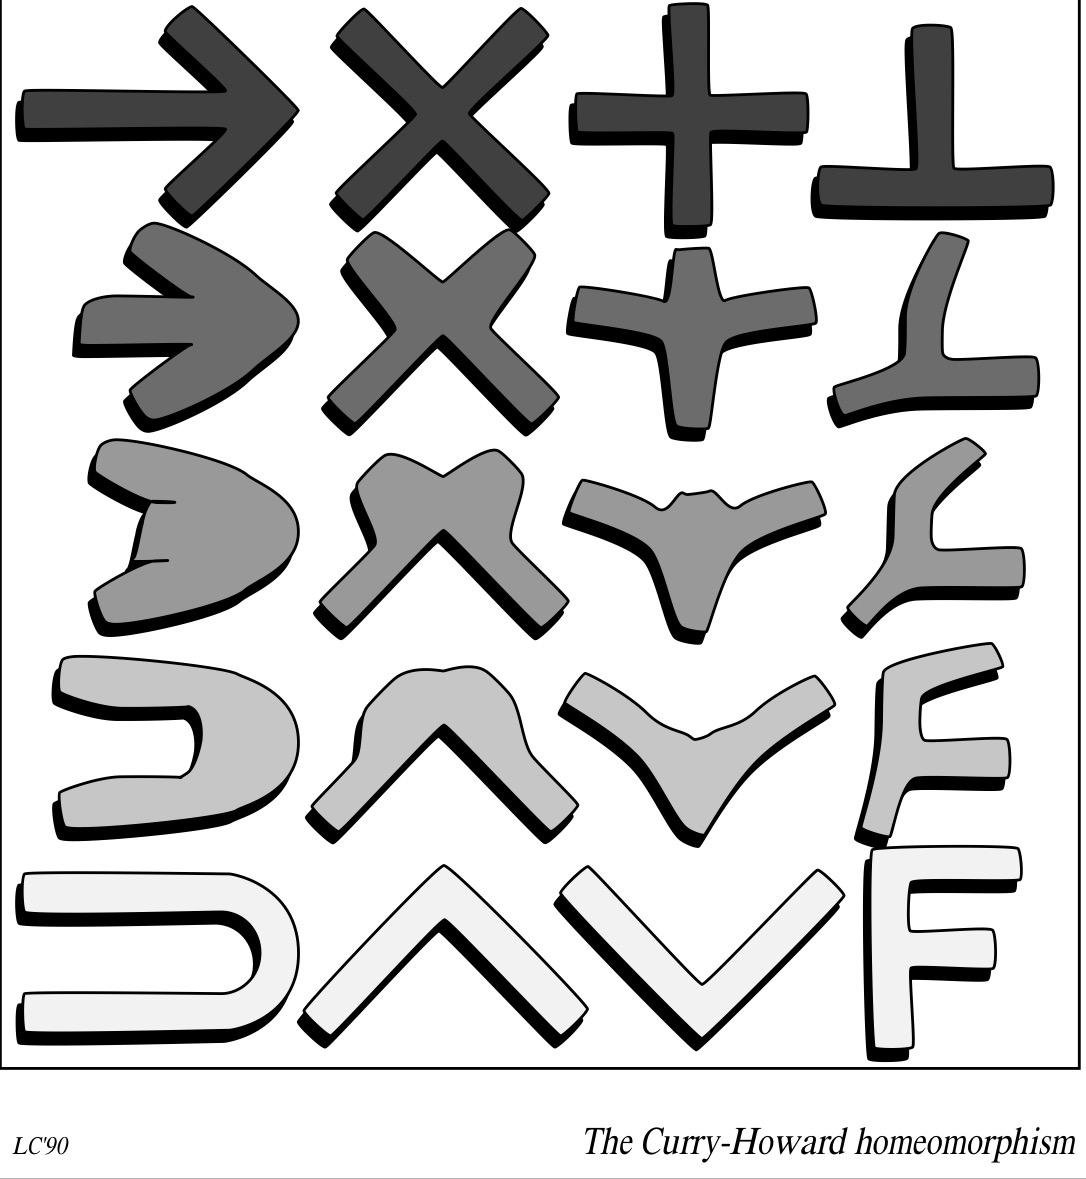
\includegraphics[scale=0.1]{cardelli-hc-corr.jpg}
      {{\tiny Source: \url{http://lucacardelli.name/Artifacts/Drawings/CurryHoward/CurryHoward.pdf}}}
    \end{figure}
\end{center}
\end{frame}

\begin{frame}[c]
  \frametitle{Background Work: Second Order Intuitionistic Propositional Logic}
  \begin{center}
    \uncover<2->{{\LARGE \color{red}Propositions are truth values not resources}}\\
    \uncover<1->{
        \fbox{Language}
        \begin{flalign*}
          \text{Propostions \& connectives}\quad A, B, C &::= x \mid A \supset B \mid \forall x. B \mid A \vee B \mid A \wedge B \\
          \text{Context}\quad \Gamma,\Delta &::= \epsilon \mid \Gamma, A
        \end{flalign*}
        \fbox{Implicit Structural Rules}

        \begin{tabular}[h]{c c c}
          $A, B \vdash A$ &  $A, B \vdash B$   & Contraction \\

          \multicolumn{2}{c}{$A \vdash A \wedge A$} & Weakening \\

          \multicolumn{2}{c}{$A, B \vdash B, A$} & Exchange
        \end{tabular}

      }
  \end{center}
\end{frame}

% \begin{frame}[c]
%   \frametitle{Background Work: Second Order Intuitionistic Propositional Logic}
%   \begin{center}
%     \uncover<2->{\LARGE {\color{red}Propositions are truth values not resources}}\\
%     \uncover<1->{{\small
%         \fbox{Language}
%         \begin{flalign*}
%           \text{Propostions \& connectives}\quad A, B, C &::= x \mid A \supset B \mid \forall x. B \mid ... \\
%           \text{Context}\quad \Gamma,\Delta &::= \epsilon \mid \Gamma, A
%         \end{flalign*}
%         \fbox{Logic Rules}
%         \begin{figure}[h]\centering
%           % ID
%           \begin{minipage}{0.20\linewidth}
%             \begin{prooftree}
%               \AxiomC{$A \in \Gamma $}\RightLabel{[Ax]}
%               \UnaryInfC{$\Gamma \vdash A $}
%             \end{prooftree}
%           \end{minipage}

%           % \forall I
%           \begin{minipage}{0.5\linewidth}
%             \begin{prooftree}
%               \AxiomC{$\Gamma \vdash B$}
%               \AxiomC{$x \notin \Gamma$}\RightLabel{[$\forall$I]}
%               \BinaryInfC{$\Gamma \vdash \forall x. B$}
%             \end{prooftree}
%           \end{minipage}\hfill%
%           % \forall E
%           \begin{minipage}{0.5\linewidth}
%             \begin{prooftree}
%               \AxiomC{$\Gamma \vdash \forall x. B$}
%               \AxiomC{$\Gamma \vdash A$}\RightLabel{[$\forall$E]}
%               \BinaryInfC{$\Gamma \vdash B[x/A]$}
%             \end{prooftree}
%           \end{minipage}

%           % -> I
%           \begin{minipage}{0.5\linewidth}
%             \begin{prooftree}
%               \AxiomC{$\Gamma,A \vdash B$}\RightLabel{[$\supset$I]}
%               \UnaryInfC{$\Gamma \vdash A \supset B$}
%             \end{prooftree}
%           \end{minipage}\hfill%
%           % -> E
%           \begin{minipage}{0.5\linewidth}
%             \begin{prooftree}
%               \AxiomC{$\Gamma \vdash A \supset B$}
%               \AxiomC{$\Gamma \vdash A$}\RightLabel{[$\supset$E]}
%               \BinaryInfC{$\Gamma \vdash B $}
%             \end{prooftree}
%           \end{minipage}
%         \end{figure}
%       }
%     }
%   \end{center}
% \end{frame}


% \begin{frame}[c]
%   \frametitle{Background Work: Substructural Logic}
%   \begin{center}
%     \begin{itemize}
%     \item<1-> Structural rules implicit in intuitionistic propositional logics\\
%       % WKN
%       \begin{minipage}{0.33\linewidth}
%         \begin{prooftree}
%           \AxiomC{$\Gamma \vdash B$}\RightLabel{[WKN]}
%           \UnaryInfC{$\Gamma, A \vdash B$}
%         \end{prooftree}
%       \end{minipage}\hfill%
%       % CTR
%       \begin{minipage}{0.33\linewidth}
%         \begin{prooftree}
%           \AxiomC{$\Gamma, A, A \vdash B$}\RightLabel{[CTR]}
%           \UnaryInfC{$\Gamma, A \vdash B $}
%         \end{prooftree}
%       \end{minipage}\hfill%
%       % EXCH
%       \begin{minipage}{0.33\linewidth}
%         \begin{prooftree}
%           \AxiomC{$\Gamma, \Delta \vdash B$}\RightLabel{[EXCH]}
%           \UnaryInfC{$\Delta, \Gamma \vdash B $}
%         \end{prooftree}
%       \end{minipage}

%     \item <2-> Control the use of [WKN] and [CTR]\\
%     \end{itemize}
%     \uncover<2->{\LARGE \color{red} Propositions now behave like resources}
%   \end{center}
% \end{frame}

\begin{frame}[c]
  \frametitle{Background Work: Substructural Logic}
  \begin{center}
{\small     \begin{tabular}[h]{c c c c}
      System                                                                                 &  Who             & Year         & Control\\ \hline\hline
      Revelance Logic\footnote[frame]{{\tiny \fullcite{orlov_relevence_1928}}}               & Orlev            & 1928         & [WKN]\\
      Lambek Logic\footnote[frame]{{\tiny \fullcite{lambek_mathematics_1958}}}               & Lambek           & 1958         & [EXCH]\\
      Affine Logic\footnote[frame]{{\tiny \fullcite{grishin_affine_1974}}}                         & Grishin          & 1974         & [CTR] \\
      Linear Logic\footnote[frame]{{\tiny \fullcite{girard_linear_1987}}}                    & Girard           & 1987         & [WKN] [CTR]\\
      \color{red}{Logic of Bunched Implications}\footnote[frame]{{\tiny \fullcite{ohearn_logic_1999}}}    & \color{red}{O'Hearn and Pym}  & \color{red}{1999} & \color{red}{[WKN] [CTR]}\\
      Separation Logic \footnote[frame]{{\tiny \fullcite{reynolds_separation_2002}}}         & Reynolds         & 2002         & [WKN] [CTR] \\
      \vdots                                                                       & \vdots              & \vdots          & \vdots
    \end{tabular}
}  \end{center}
\end{frame}

\begin{frame}
  \frametitle{Background work: Logic of \BI{}}
  \begin{center}
    Coffee Shop

    1 cup coffee costs \$2

    \uncover<1->{
      \begin{tabular}[c]{c c c c c}
        \raisebox{-0.4\height}{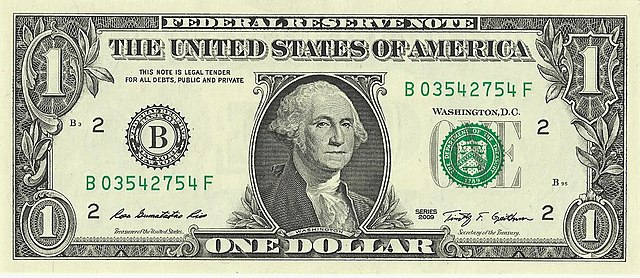
\includegraphics[scale=0.15]{one_usd}}
        & {\LARGE $,$}
        & \raisebox{-0.4\height}{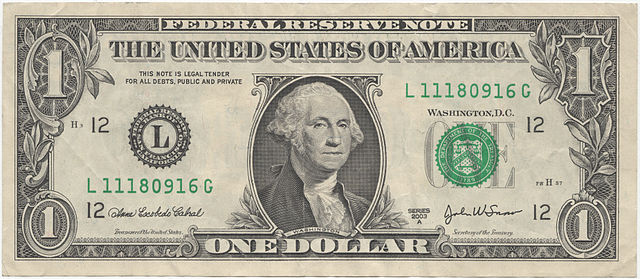
\includegraphics[scale=0.151]{one_usd_2}}
        & {\LARGE $\vdash$}
        & \raisebox{-0.4\height}{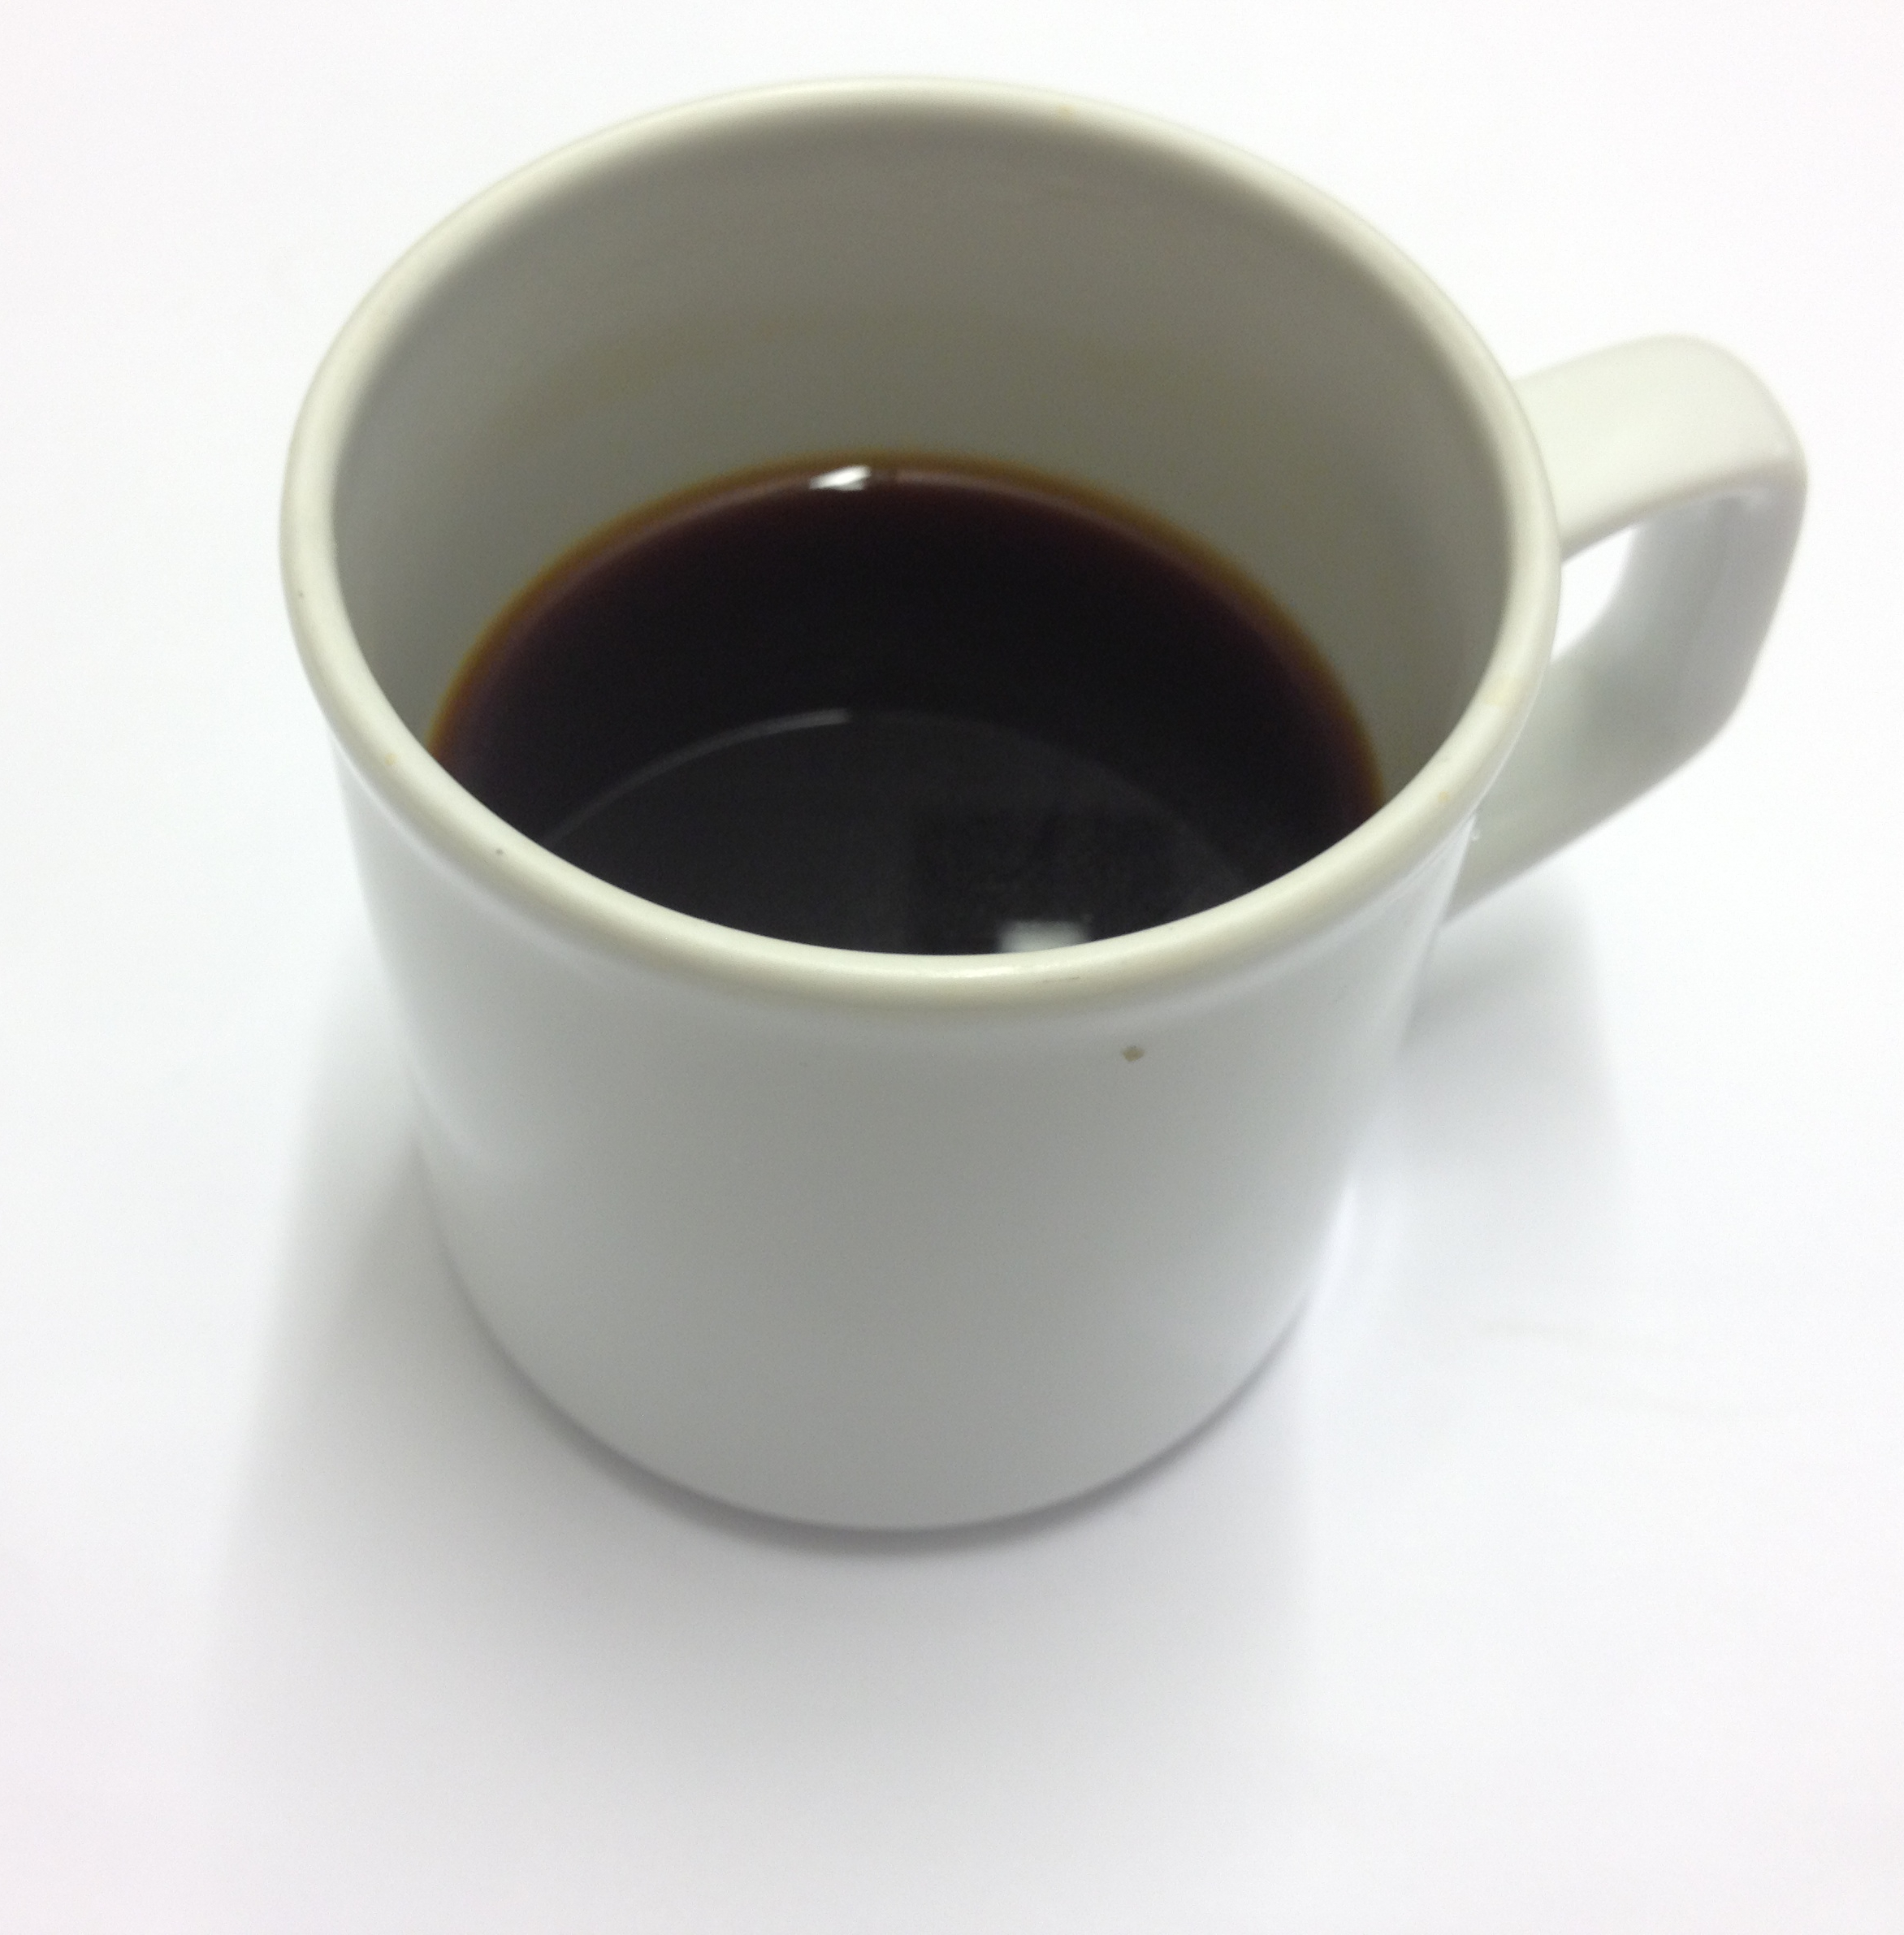
\includegraphics[scale=0.03]{coffee_cup}}
      \end{tabular}
    }
    \uncover<2->{
      \begin{tabular}[c]{c c c c c}
        \raisebox{-0.4\height}{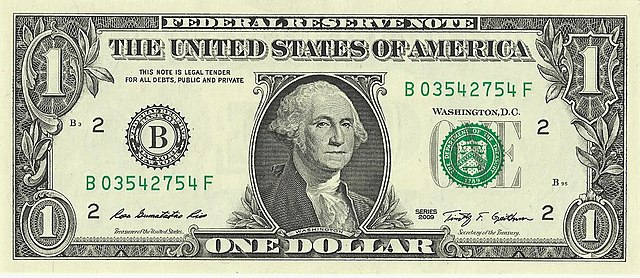
\includegraphics[scale=0.15]{one_usd}}
        & {\LARGE $,$}
        & \raisebox{-0.4\height}{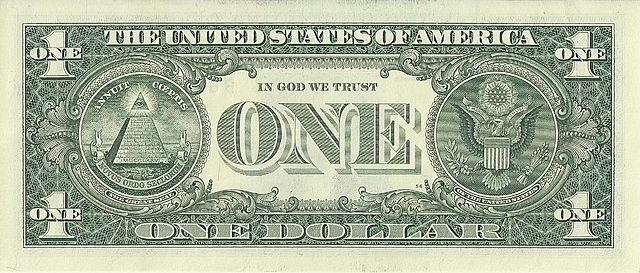
\includegraphics[scale=0.2]{one_usd_rev}}
        & {\LARGE $\not\vdash$}
        & \raisebox{-0.4\height}{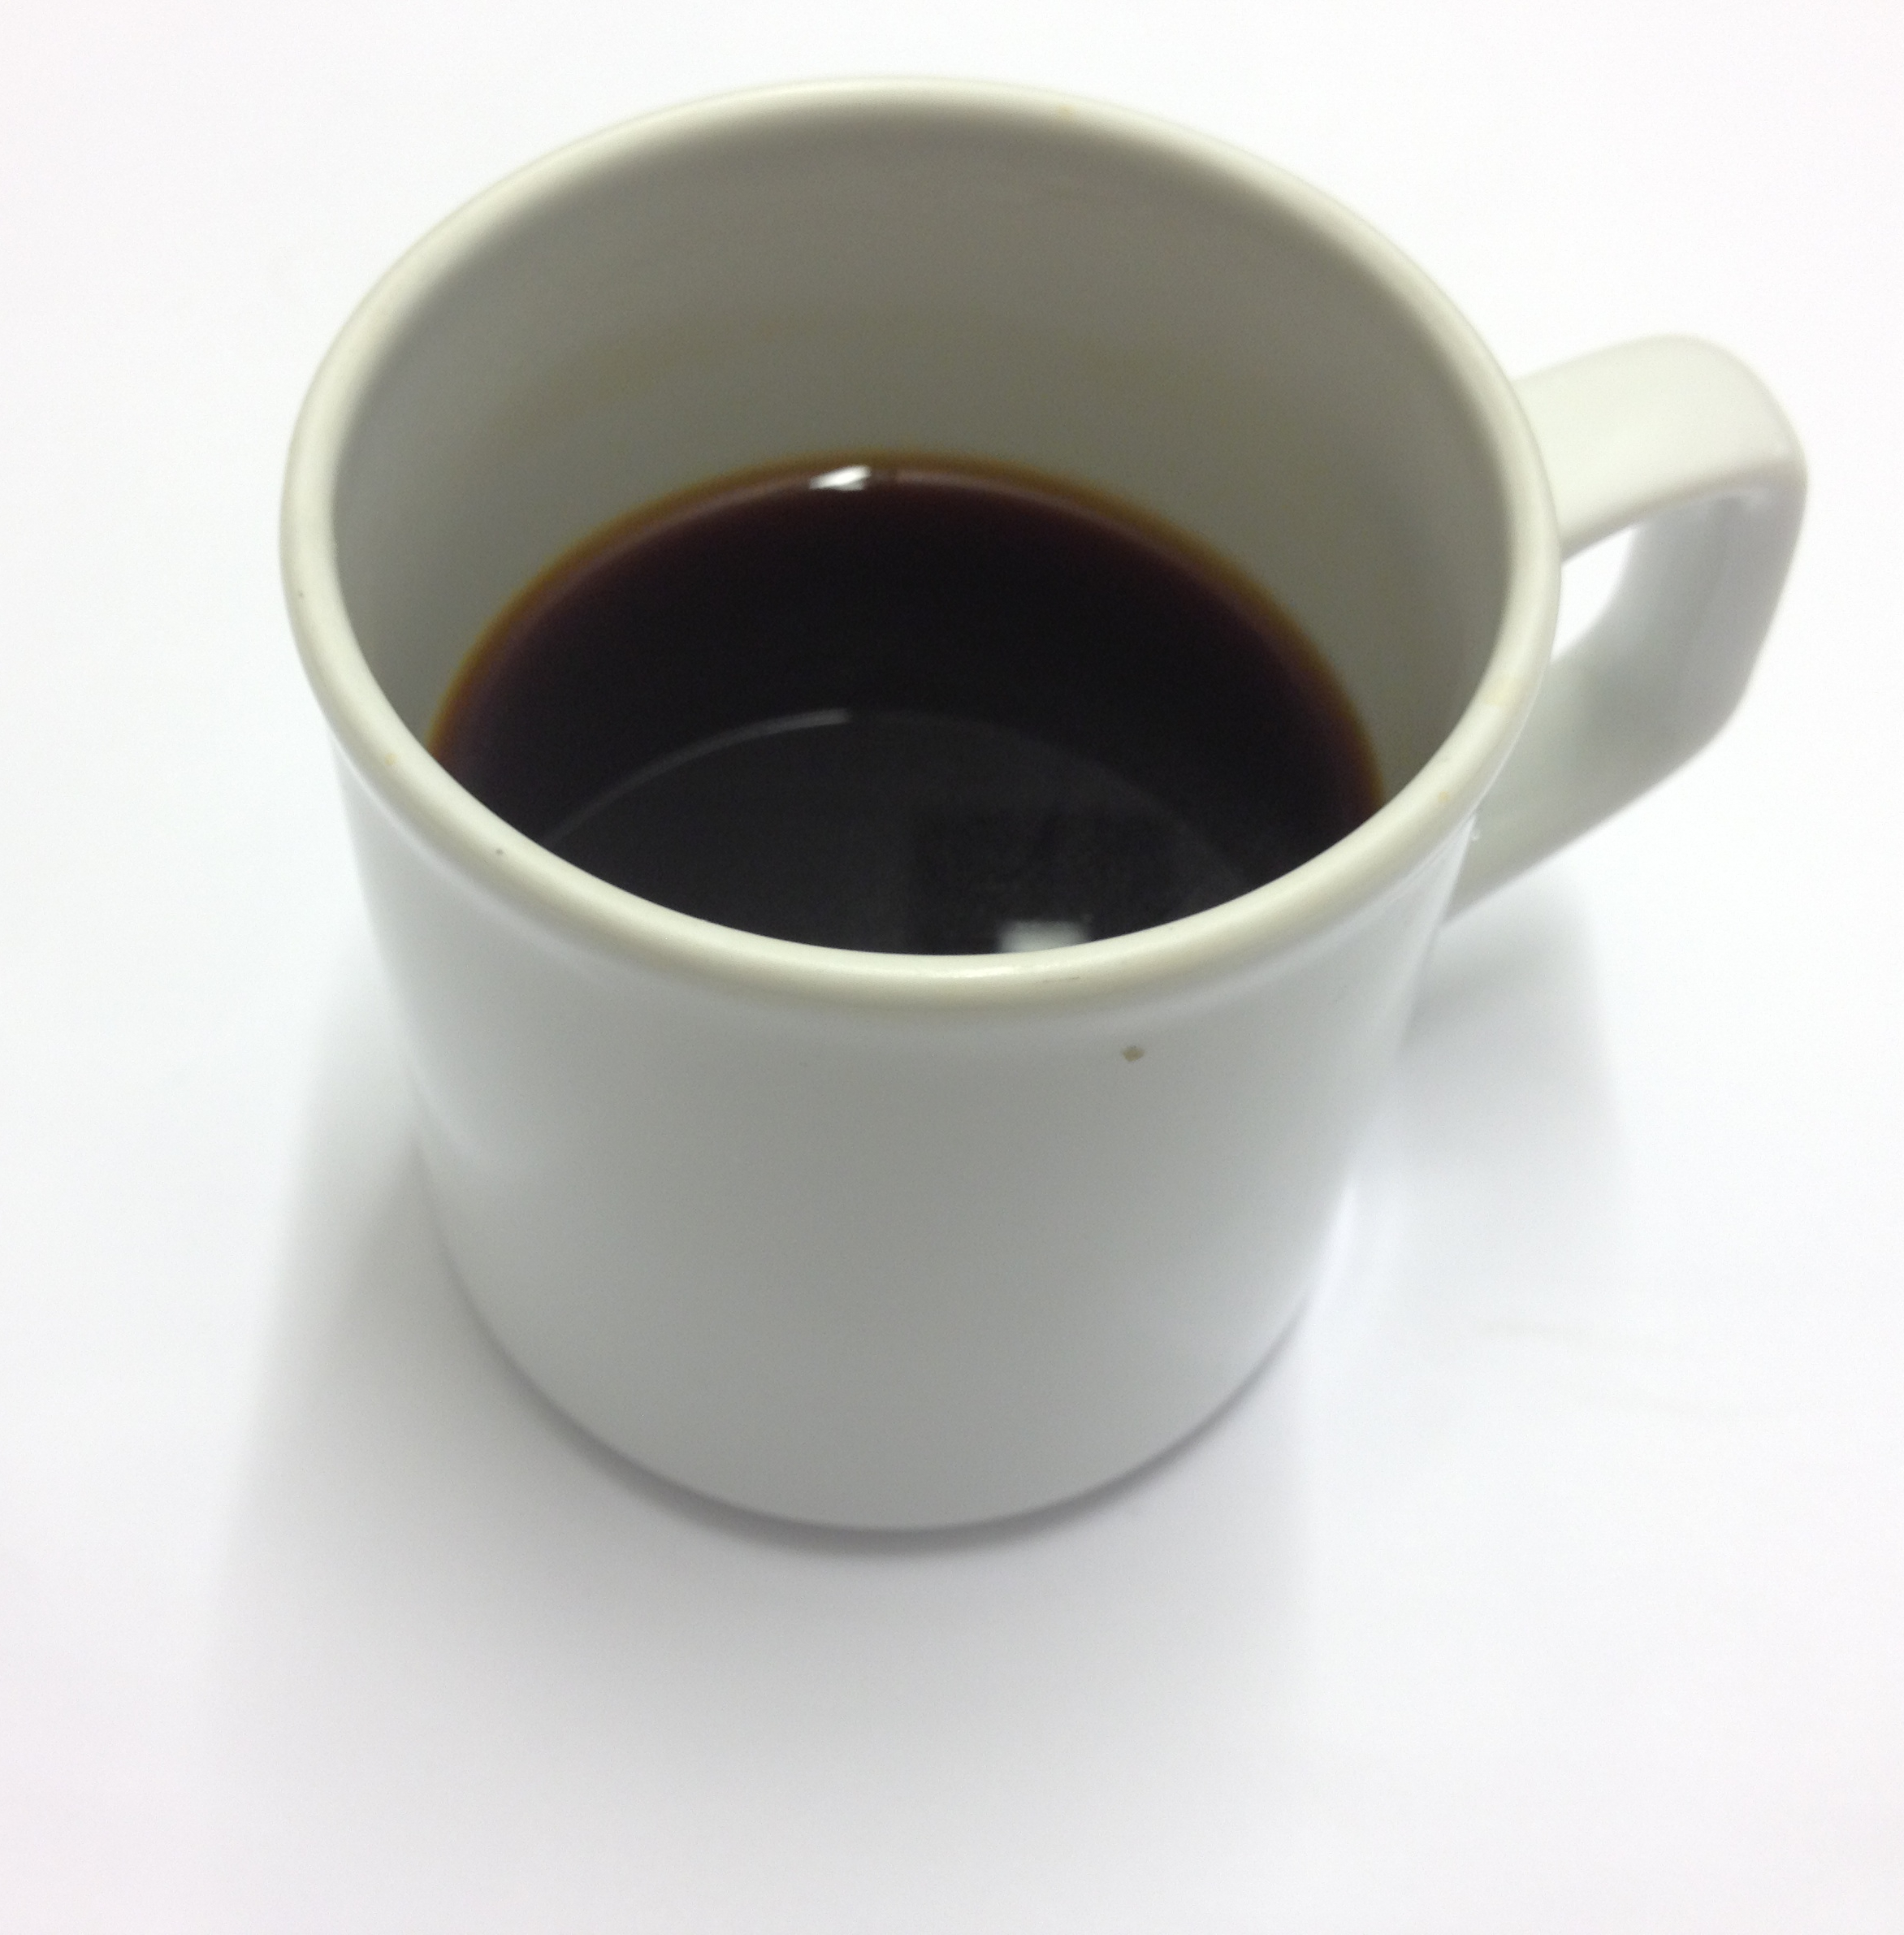
\includegraphics[scale=0.03]{coffee_cup}}
      \end{tabular}

      {\color{red}two separate} dollar bills necessary
    }
  \end{center}
\end{frame}

\begin{frame}[c]
  \frametitle{Background Work: Logic of \BI{}}
  \begin{center}
    \begin{itemize}

    \item<1-> Conjunction ($\wedge$) split into two flavors
      \begin{center}
      \begin{tabular}[c]{c l}
      $A \otimes B$& A is separate from B\\
      $A \with B$&  A is a different view of B or A shares with B
      \end{tabular}
    \end{center}
    \item<2-> \BI{} contexts sensitive to different conjunction
      \begin{center}
        \begin{minipage}[h]{0.5\linewidth}
          $A, B \vdash A \otimes B$
        \end{minipage}%
        \begin{minipage}[h]{0.5\linewidth}
          $A; B \vdash A \with B$
        \end{minipage}
    \end{center}
    \item<3-> Contexts form trees, called bunches
      \begin{center}
        \begin{figure}[h]\centering
      \begin{minipage}{0.5\linewidth}\centering
        \tikzset{every tree node/.style={minimum width=2em},
          blank/.style={draw=none},
          edge from parent/.style=
          {draw,edge from parent path={(\tikzparentnode) -- (\tikzchildnode)}},
          level distance=1.5cm}
        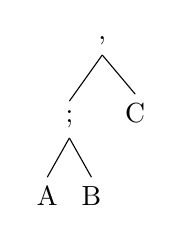
\begin{tikzpicture}
          \Tree
          [.,
          [.;
          [.A ]
          [.B ]
          ]
          [.C ]
          ]
        \end{tikzpicture}
        \caption*{$(A;B),C$}
      \end{minipage}%
      \begin{minipage}{0.5\linewidth}\centering
        \tikzset{every tree node/.style={minimum width=2em},
          blank/.style={draw=none},
          edge from parent/.style=
          {draw,edge from parent path={(\tikzparentnode) -- (\tikzchildnode)}},
          level distance=1.5cm}
        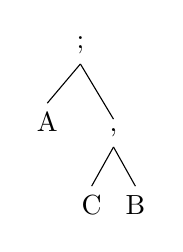
\begin{tikzpicture}
          \Tree
          [.;
          [.A ]
          [.,
          [.C ]
          [.B ]
          ]
          ]
        \end{tikzpicture}
        \caption*{$A;(B,C)$}
      \end{minipage}
    \end{figure}

    \end{center}

\end{itemize}
\end{center}
\end{frame}

\begin{frame}[c]
  \frametitle{Background Work: Logic of \BI{}}
  \begin{center}
  Context connectives guide structural rules

  \begin{itemize}
  \item Contraction
    \begin{center}
      $A \vdash A;A$\\
      $A \not\vdash A,A$
    \end{center}

  \item Weakening
    \begin{center}
      $A;A \vdash A$ \qquad $A;B \vdash B$ \qquad $A;B \vdash A$\\
      $A,B \not\vdash A$ \qquad $A,B \not\vdash B$
    \end{center}
  \end{itemize}
\end{center}
\end{frame}

\begin{frame}[c]
  \frametitle{Background Work: Logic of \BI{}}
  \begin{center}
    Implications naturally get corresponding flavors

    $A \otimes B \vdash C\ \text{iff}\ A \vdash B \sepimp C$

    $A \with B \vdash C\ \text{iff}\ A \vdash B \shimp C$
  \end{center}
\end{frame}

\begin{frame}
  \frametitle{Background work: Logic of \BI{}}
  \begin{center}
    Coffee Shop (Revisited)

    1 cup coffee costs \$2 \qquad  1 cookie costs \$1
    \begin{tabular}[c]{c c c c c}
        \raisebox{-0.4\height}{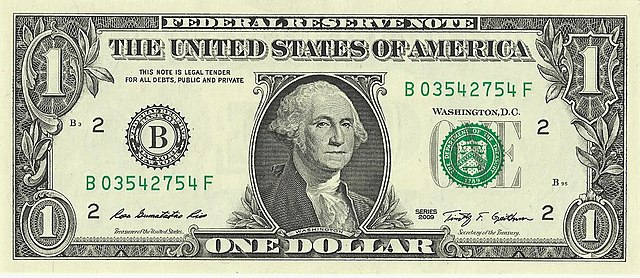
\includegraphics[scale=0.12]{one_usd}}
        & {\LARGE $\vdash$}
        & \raisebox{-0.4\height}{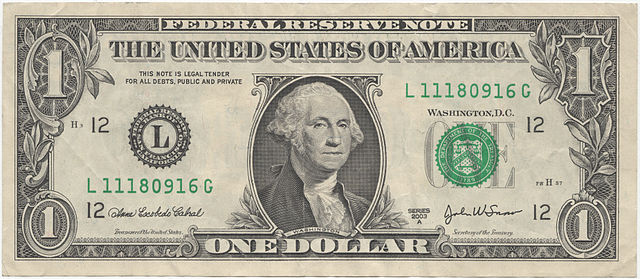
\includegraphics[scale=0.121]{one_usd_2}}
        & {\LARGE $\sepimp$}
        & \raisebox{-0.4\height}{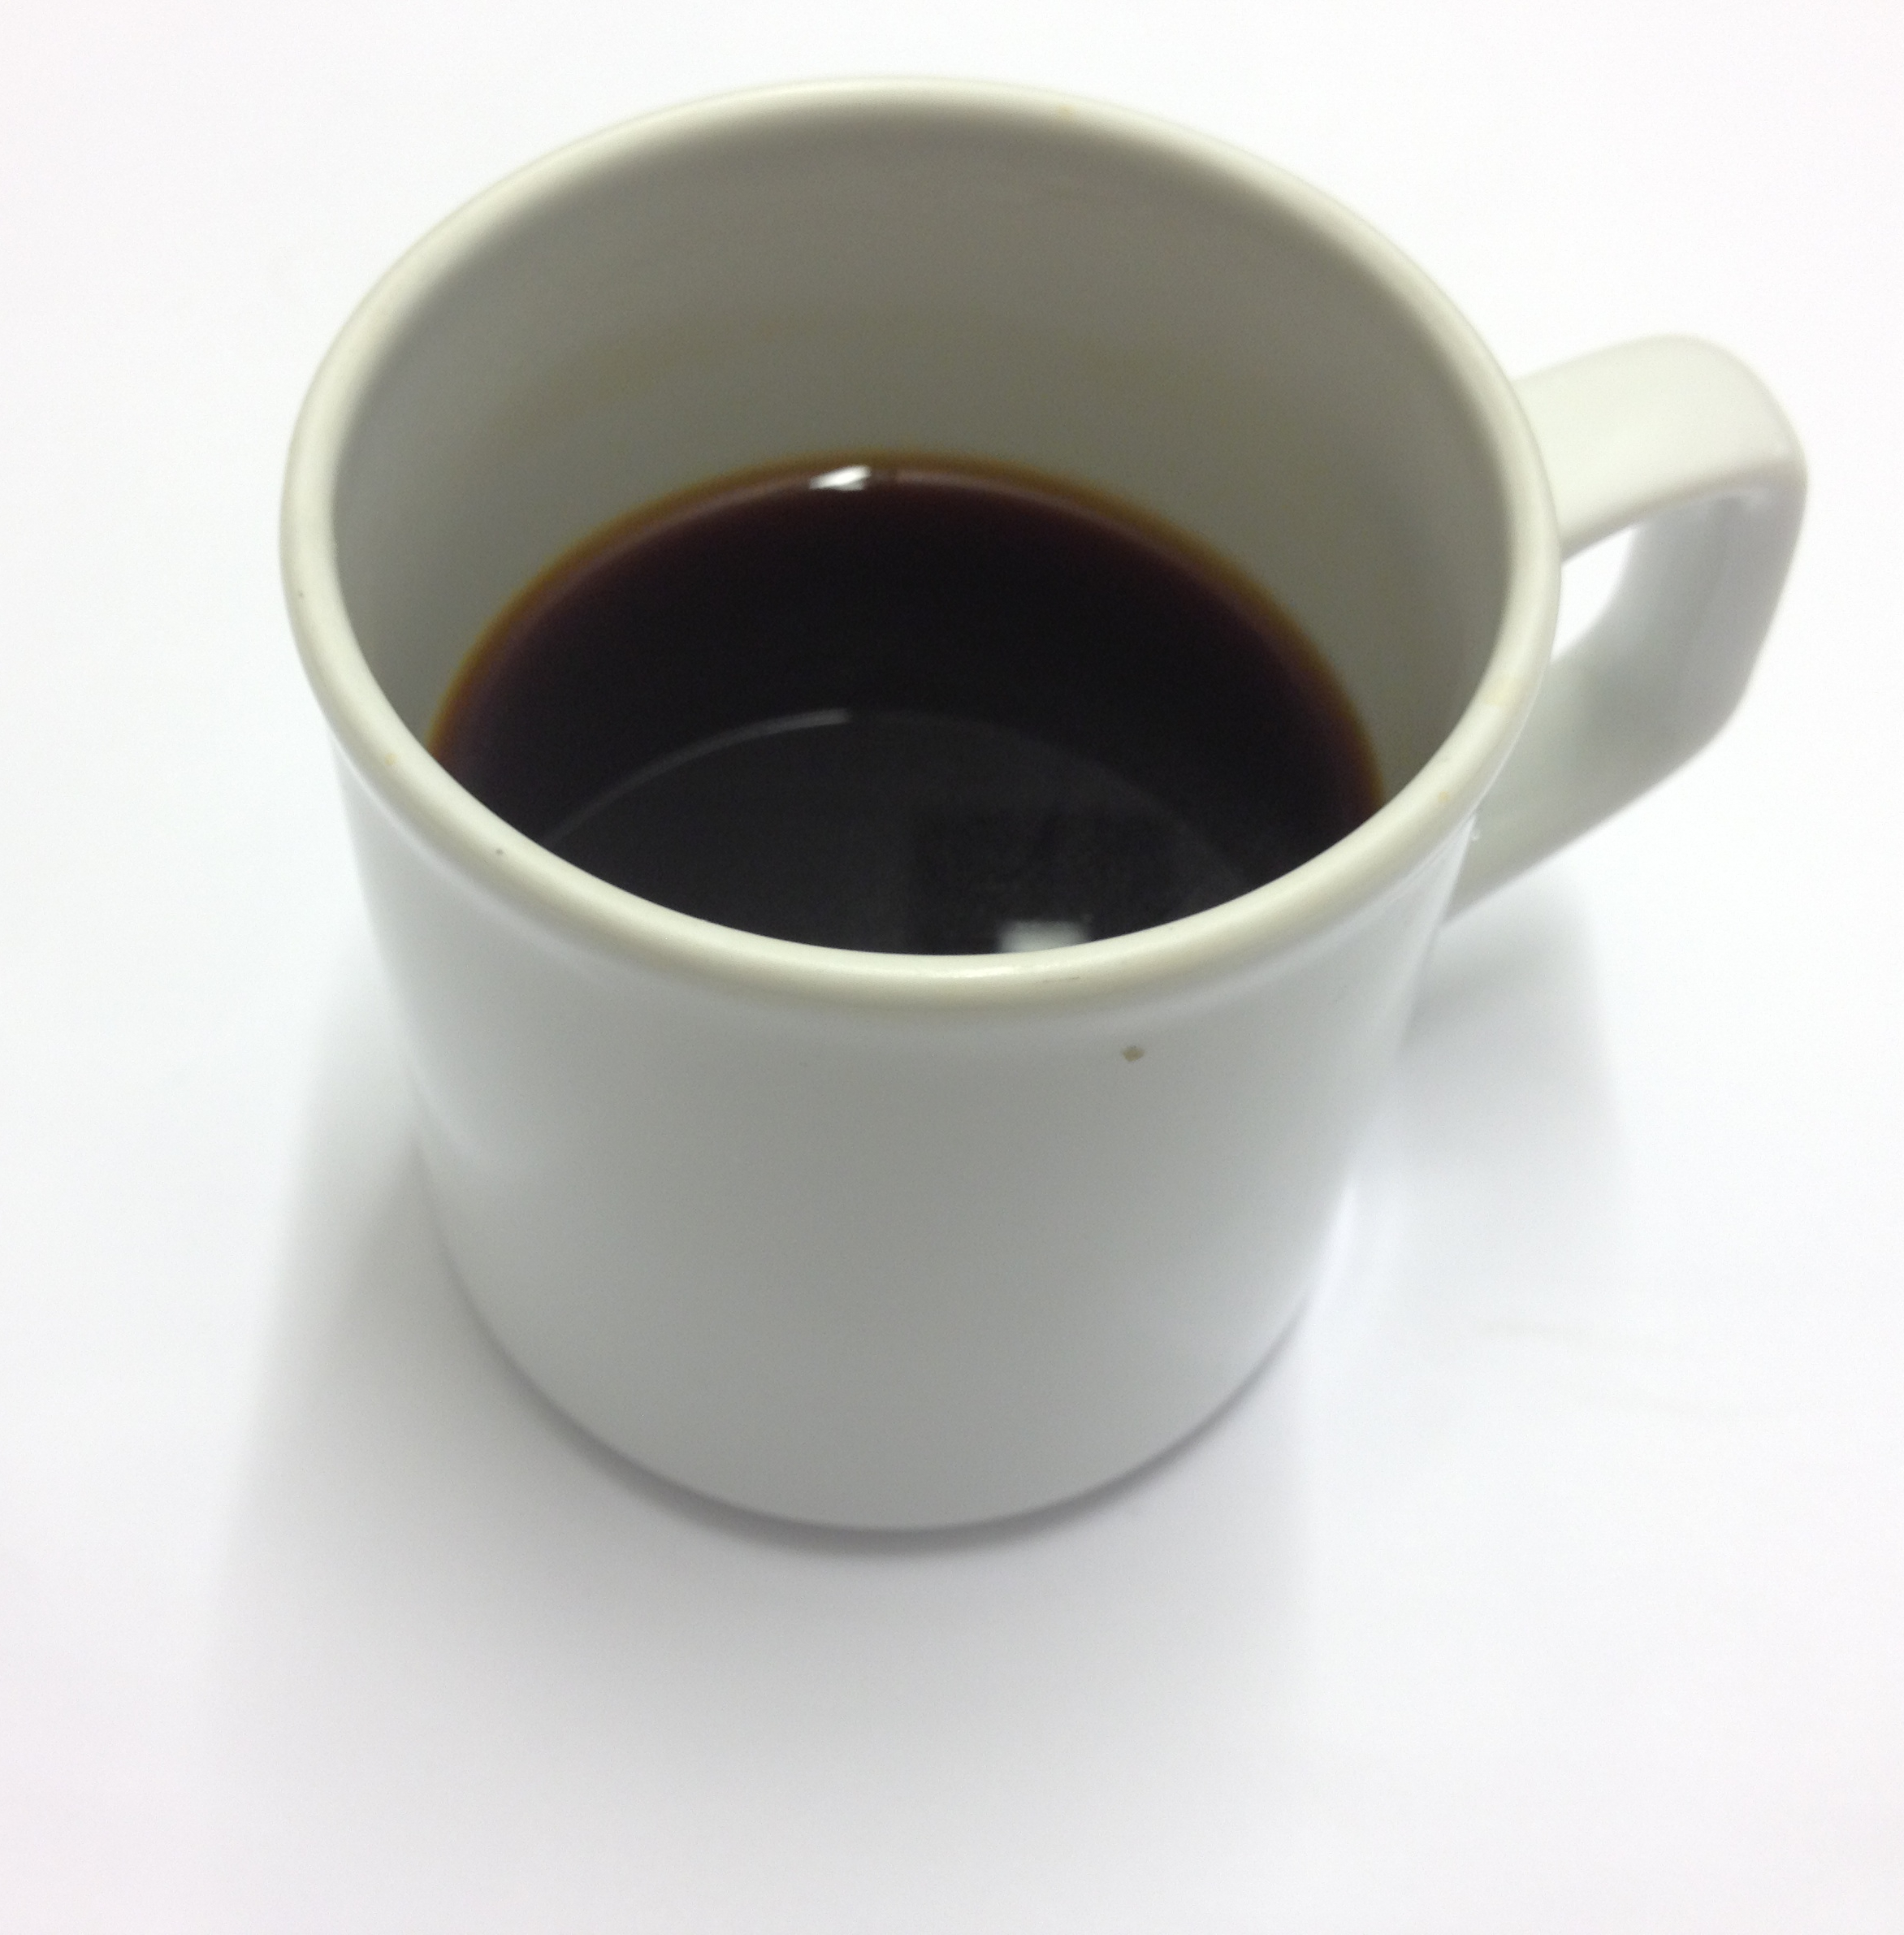
\includegraphics[scale=0.025]{coffee_cup}}
      \end{tabular}

      \begin{tabular}[c]{c c c c c}
        \raisebox{-0.4\height}{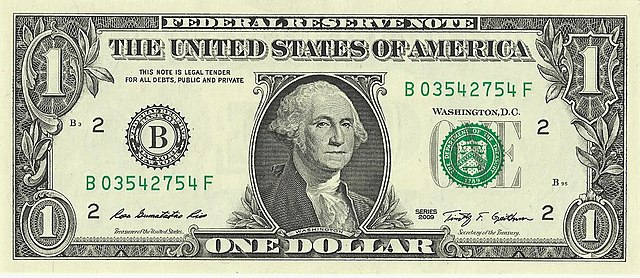
\includegraphics[scale=0.12]{one_usd}}
        & {\LARGE $\vdash$}
        & \raisebox{-0.4\height}{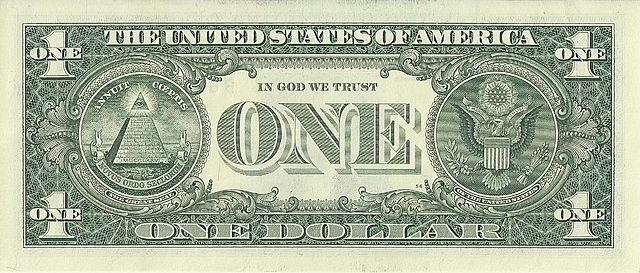
\includegraphics[scale=0.16]{one_usd_rev}}
        & {\LARGE $\shimp$}
        & \raisebox{-0.4\height}{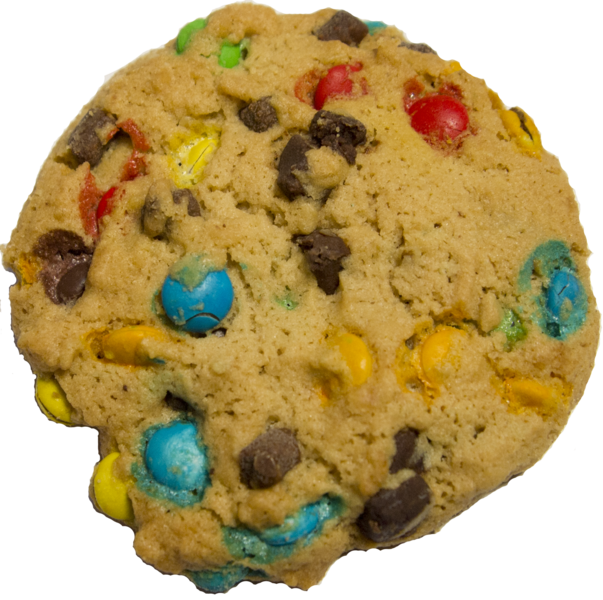
\includegraphics[scale=0.25]{cookie}}
      \end{tabular}

      \begin{tabular}[c]{c c c c c}
        \raisebox{-0.4\height}{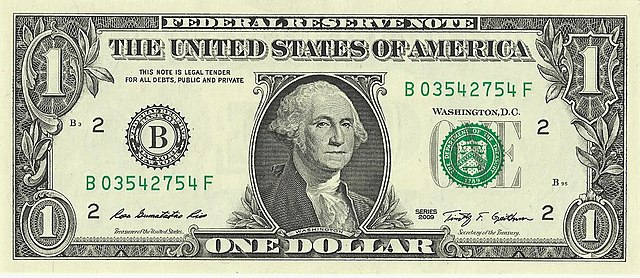
\includegraphics[scale=0.12]{one_usd}}
        & {\LARGE $\not\vdash$}
        & \raisebox{-0.4\height}{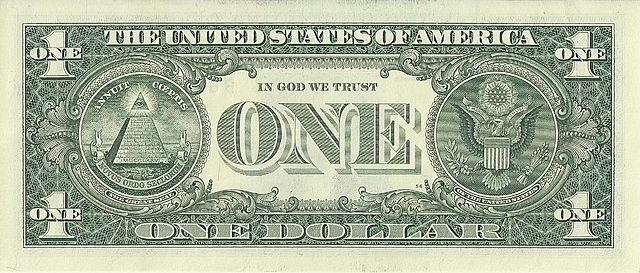
\includegraphics[scale=0.17]{one_usd_rev}}
        & {\LARGE $\shimp$}
        & \raisebox{-0.4\height}{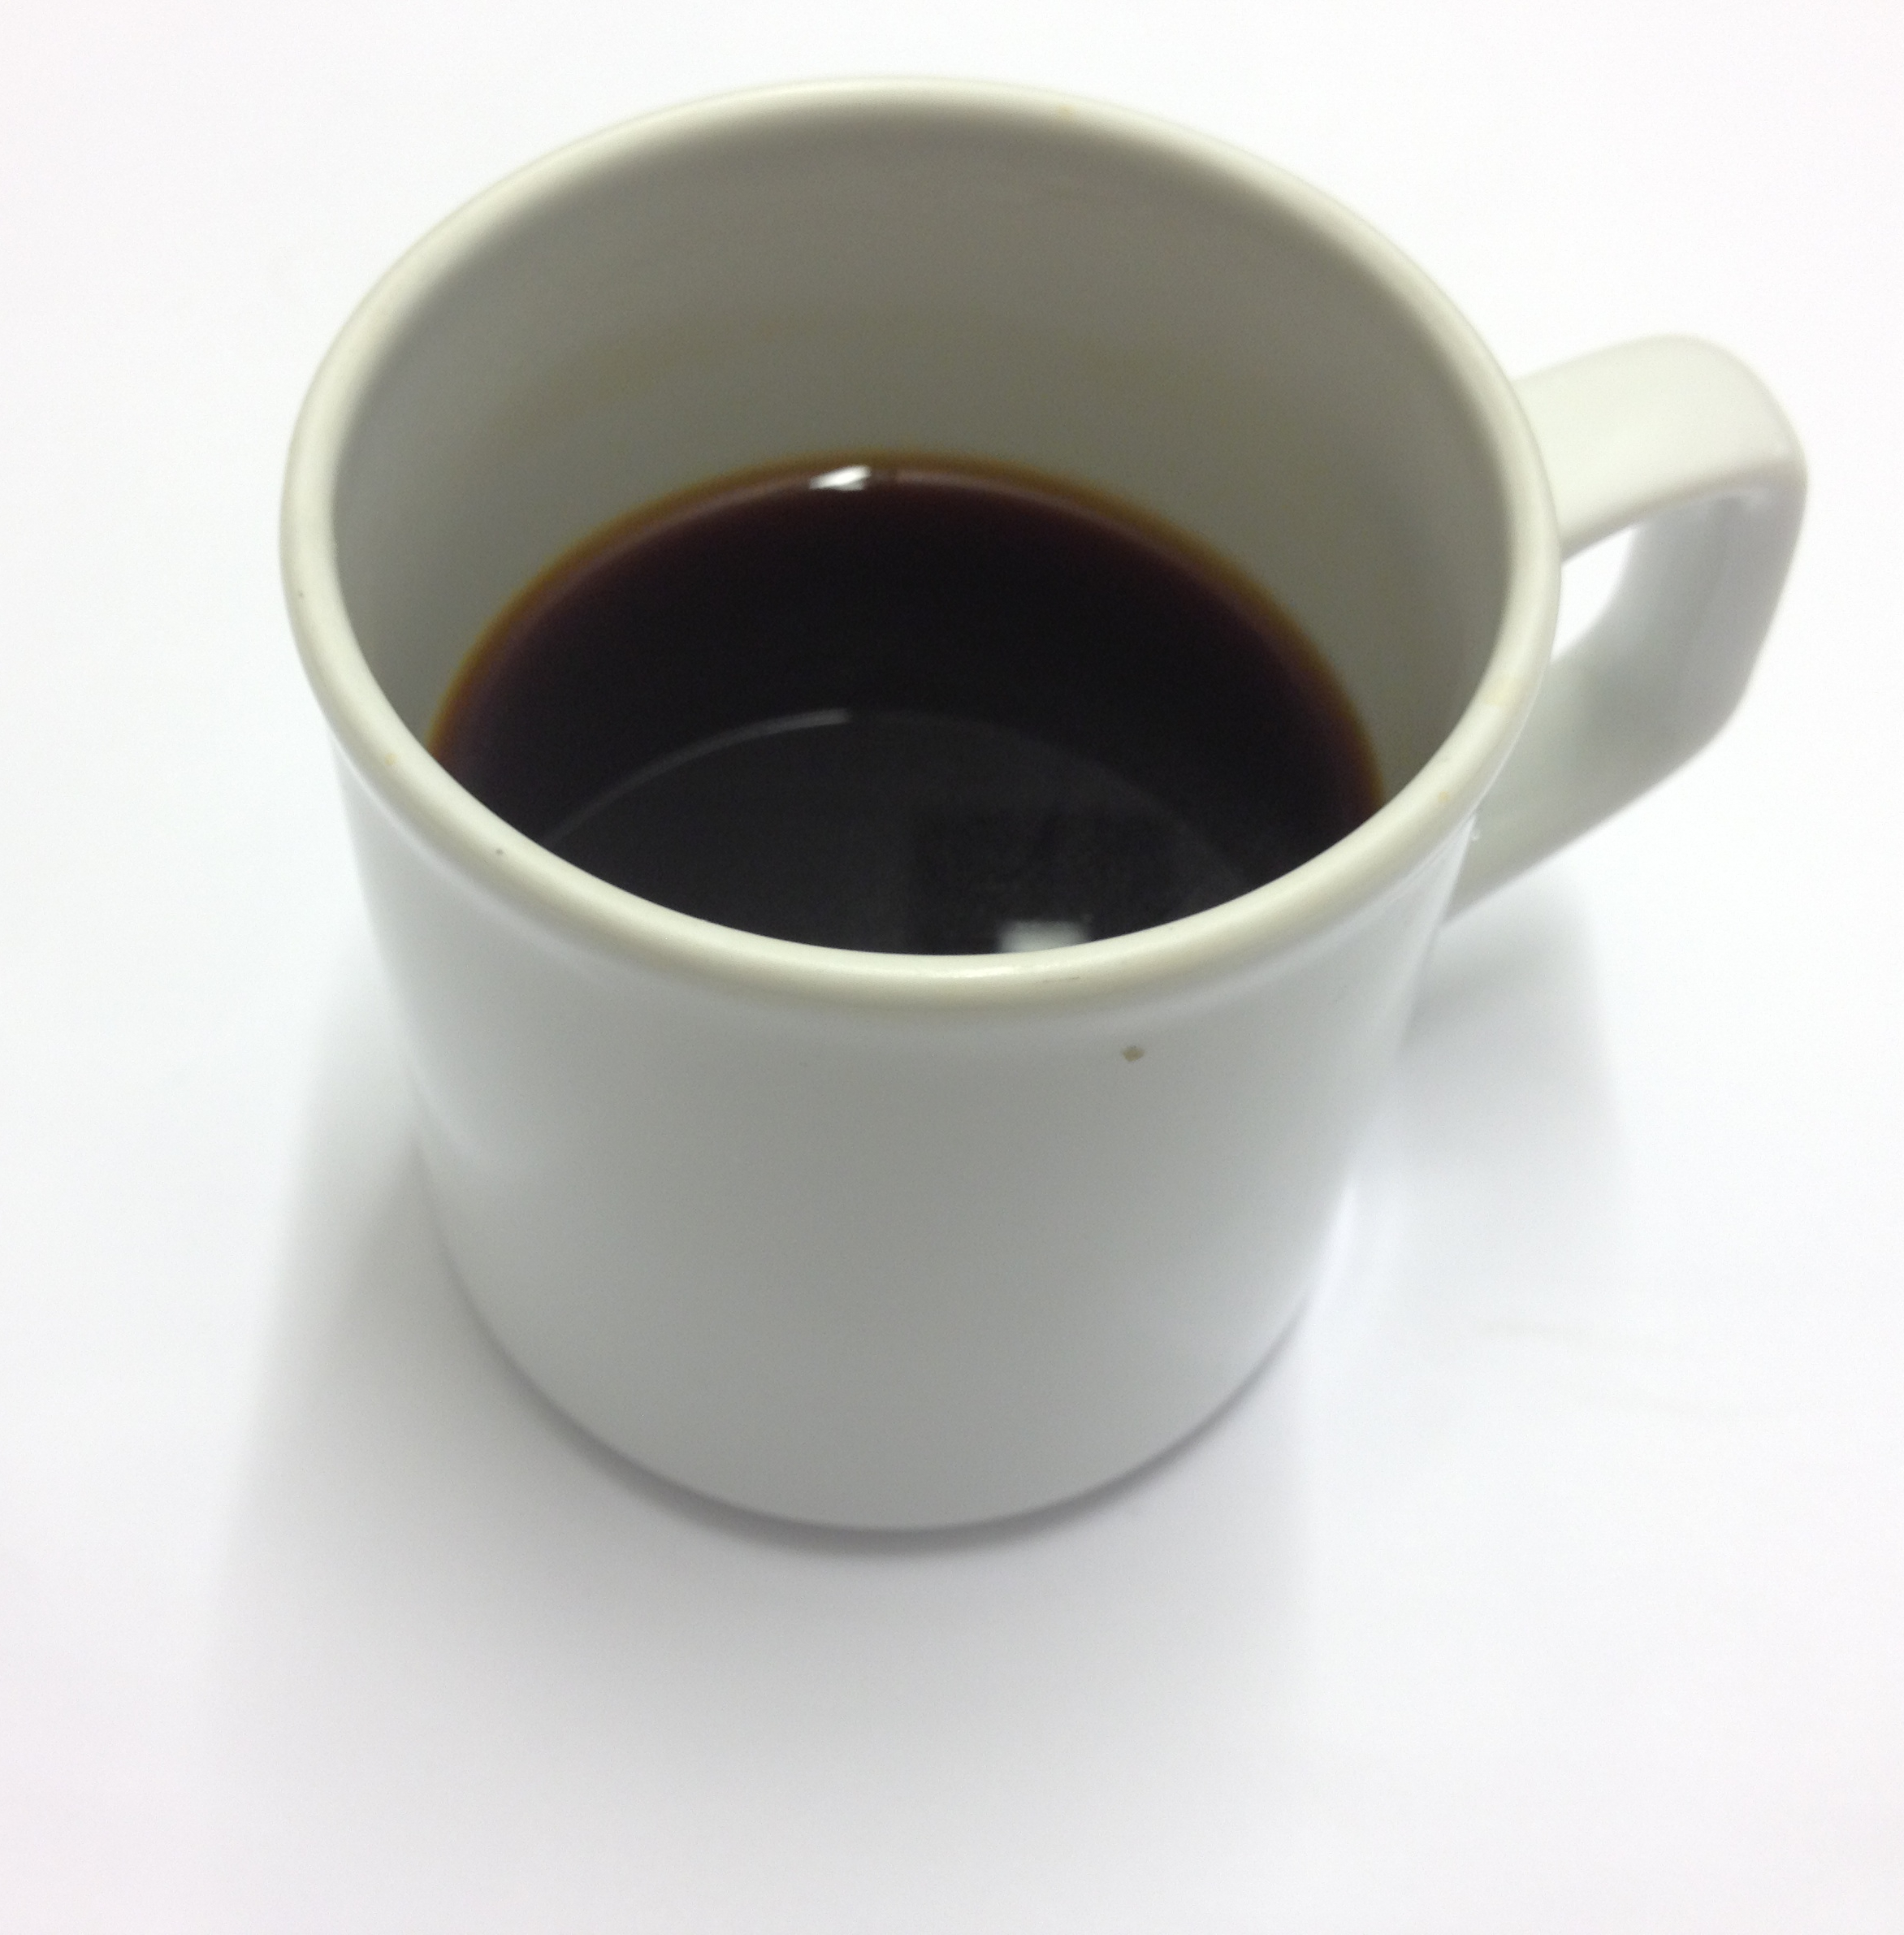
\includegraphics[scale=0.025]{coffee_cup}}
      \end{tabular}

  \end{center}
\end{frame}


%%% Local Variables:
%%% mode: latex
%%% TeX-master: "defense-slides"
%%% End:


% Qub
% 10 mins
\section{\qub{}}\label{sec:qub}
% (10 min)

\begin{frame}
  \frametitle{\qub{}}
  \begin{center}
    \begin{itemize}
    \item Quill: {\color{blue}Qu}al{\color{blue}i}fied types + {\color{blue}l}inear {\color{blue}l}ogic\\
    \item \qub{}: {\color{blue}Qu}alified types + logic of {\color{blue}b}unched implications 
    \end{itemize}
  \end{center}
\end{frame}

\begin{frame}
  \frametitle{\qub{}: Types and Predicates}
  \begin{center}
      \begin{minipage}{0.65\linewidth}
    \begin{flalign*}
      \text{Types}\ \ \  \tau, \upsilon, \phi         &::= t \mid \iota \mid \tau \rightarrow \tau\\
                   &\text{where}\qquad \rightarrow \in \{\tightoverset{\scalebox{0.5}{!}}{\sepimp}, \sepimp, \tightoverset{\scalebox{0.5}{!}}{\shimp}, \shimp \}\\
      \text{Predicates}\ \ \        \pi,\omega        &::= \texttt{Un}\ \tau \mid \texttt{SeFun}\ \tau \mid \texttt{ShFun}\ \tau \mid \tau \geq \tau' \\
      \text{Qualified Types}\ \ \     \rho            &::= \tau \mid \pi => \rho \\
      \text{Type schemes}\ \ \        \sigma          &::= \rho \mid \forall t. \sigma
    \end{flalign*}
  \end{minipage}
  \begin{itemize}
  \item $\SeFun{\tau}$: $\tau$ is a function that is separate from its argument
  \item $\ShFun{\tau}$: $\tau$ is a function that is in sharing with its argument
  \item $\Un{\tau}$: $\tau$ does not have resources or they can be copied/dropped easily
  \end{itemize}
  \end{center}
\end{frame}


\begin{frame}
  \frametitle{\qub{}: Types and Predicates}
  \begin{center}
      \begin{minipage}{0.65\linewidth}
    \begin{flalign*}
      \text{Types}\ \ \  \tau, \upsilon, \phi         &::= t \mid \iota \mid \tau \rightarrow \tau\\
                   &\text{where}\qquad \rightarrow \in \{\tightoverset{\scalebox{0.5}{!}}{\sepimp}, \sepimp, \tightoverset{\scalebox{0.5}{!}}{\shimp}, \shimp \}\\
      \text{Predicates}\ \ \        \pi,\omega        &::= \texttt{Un}\ \tau \mid \texttt{SeFun}\ \tau \mid \texttt{ShFun}\ \tau \mid \tau \geq \tau' \\
      \text{Qualified Types}\ \ \     \rho            &::= \tau \mid \pi => \rho \\
      \text{Type schemes}\ \ \        \sigma          &::= \rho \mid \forall t. \sigma
    \end{flalign*}
  \end{minipage}
  \begin{itemize}
  \item $\sepimp$: Function type that is separate with its argument
  \item $\shimp$: Function type that is in sharing with its argument
  \item $\tightoverset{\scalebox{0.5}{!}}{\sepimp}$, $\tightoverset{\scalebox{0.5}{!}}{\shimp}$: unrestriced versions of $\sepimp$ and $\shimp$
  \end{itemize}
  \end{center}
\end{frame}

\begin{frame}
  \frametitle{\qub{}: Language}
  \begin{center}
    \begin{flalign*}
      \text{Term Variables}\ \ \  x, y, z  &\in \text{Var} \nonumber\\
      \text{Expressions}\ \ \     M, N     &::= x \mid \lambda^{\sepimp}x. M \mid \lambda^{\shimp}x. M \mid M N \mid \Let{x}{M}{N}\nonumber
    \end{flalign*}
    \begin{itemize}
    \item $\lambda^{\sepimp}x. M$: Introduces $\sepimp$ function
    \item $\lambda^{\shimp}x. N$: Introduces $\shimp$ function
    \end{itemize}
  \end{center}
\end{frame}

\begin{frame}
  \frametitle{\qub{}: Typing Environmnet}
  \begin{center}
    \begin{itemize}
    \item Logic of \BI{}: Contexts are trees
    \item \qub{}: Contexts are flattened sharing graphs
    \end{itemize}
    {\small
      \begin{minipage}[c]{0.45\linewidth}
      \centering
      \tikzset{every tree node/.style={minimum width=2em},
        blank/.style={draw=none},
        edge from parent/.style=
        {draw,edge from parent path={(\tikzparentnode) -- (\tikzchildnode)}},
        level distance=1.5cm}
      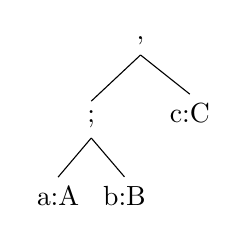
\begin{tikzpicture}
        \Tree
        [.,
        [.;
        [.a:A ]
        [.b:B ]
        ]
        [.c:C ]
        ]
      \end{tikzpicture}
    \end{minipage}\hfill%
    \begin{minipage}[c]{0.45\linewidth}
      \centering
      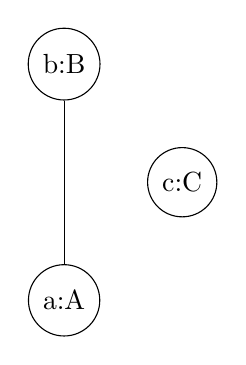
\begin{tikzpicture}
        \node[shape=circle,draw=black] (A) at (0,0) {a:A};
        \node[shape=circle,draw=black] (B) at (0,3) {b:B};
        \node[shape=circle,draw=black] (C) at (1.5,1.5) {c:C};

        \path [-] (A) edge node {} (B);
      \end{tikzpicture}
    \end{minipage}
  }
  \begin{itemize}
  \item Sharing relation $\Psi$
    \begin{flalign*}
 &\forall_{x \in \texttt{dom}(\Psi)}\ x \in \Psi(x) \tag{reflexive}\\
 &\forall_{x,y \in \texttt{dom}(\Psi)}\ \text{if}\ y \in \Psi(x)\ \text{then}\ x \in \Psi(y) \tag{symmetric}\\
 &\forall_{x,y,z \in \texttt{dom}(\Psi)}\ \text{if}\ y \in \Psi(x)\ \text{and}\ z \in \Psi(y)\ \nRightarrow z \in \Psi(x) \tag{non-transitive}
\end{flalign*}
\end{itemize}
\end{center}
\end{frame}

\begin{frame}
  \frametitle{\qub{}: Typing Environment}
  \begin{center}
    ``$x$ of type $\sigma$ is in sharing with $\vec{y}$''\\
    $(x, \sigma, \vec{y}) \in \Gamma$
    \begin{flalign*}
      \text{Typing Context}\ \ \      \Gamma,\Delta     &::= \epsilon \mid \Gamma, x^{\vec{y}}:\sigma
    \end{flalign*}
    \begin{flalign*}
      \texttt{Vars}(\Gamma, x^{\vec{y}}:\tau) &= \texttt{Vars}(\Gamma) \cup \{ x \}\\
      \texttt{Shared}(\Gamma, x^{\vec{y}}:\tau) &= \texttt{Shared}(\Gamma) \cup \{ \vec{y} \}\\
      \texttt{Used}(\Gamma) &= \texttt{Vars}(\Gamma) \cup \texttt{Shared}(\Gamma)
    \end{flalign*}
    \begin{flalign*}
      (\Gamma, x^{\vec{y}}:\tau)^{[a \mapsto \vec{b}]} &= \begin{cases}
        a \notin \vec{y}\ \ \ \ (\Gamma^{[a \mapsto \vec{b}]}, x^{\vec{y}}:\tau)\\
        a \in \vec{y}\ \ \ \  (\Gamma^{[a \mapsto \vec{b}]}, x^{(\vec{y}\backslash a)\cup\vec{b}}:\tau)
      \end{cases}\\
      \Gamma^{[\vec{a} \mapsto \vec{b}]} &= (\dots((\Gamma^{[a_1 \mapsto \vec{b}]})^{[a_2 \mapsto \vec{b}]})^{\dots})^{[a_n \mapsto \vec{b}]}
    \end{flalign*}
    \begin{flalign*}
      \Gamma \circledast \Gamma' &= \Gamma \sqcup \Gamma' \qquad
      \texttt{if}\ \texttt{Vars}(\Gamma) \mathbin{\#} \texttt{Used}(\Gamma') \wedge \texttt{Vars}(\Gamma') \mathbin{\#} \texttt{Used}(\Gamma)\\
      \Gamma \varoplus \Gamma'   &= \Gamma \sqcup \Gamma' \qquad
      \texttt{if}\ \texttt{Used}(\Gamma) = \texttt{Used}(\Gamma')
    \end{flalign*}
  \end{center}
\end{frame}

\begin{frame}
  \frametitle{\qub{}: Typing Rules}
  \begin{center}
    \fbox{Structural Rules}
    {\footnotesize
      \begin{figure}[h]\centering
    % ID
    \begin{minipage}{1\textwidth}
      \begin{prooftree}
        \AxiomC{{\color{white}$\Gamma \circledast \Delta \circledast$}} \RightLabel{[ID]}
        \UnaryInfC{$P \mid x^{\vec{y}} : \sigma \vdash x : \sigma $}
      \end{prooftree}
    \end{minipage}

    % CTR UN
    \begin{minipage}{.55\textwidth}
      \begin{prooftree}
        \AxiomC{$P \mid \Gamma \circledast \Delta \circledast \Delta \vdash M : \sigma$}
        \AxiomC{$P \vdash \Delta\ \texttt{un}$} \RightLabel{[CTR-UN]}
        \BinaryInfC{$P \mid \Gamma \circledast \Delta \vdash M : \sigma$}
      \end{prooftree}
    \end{minipage}%
    % CTR Sh
    \begin{minipage}{.45\textwidth}
      \begin{prooftree}
        \AxiomC{$P \mid \Gamma \varoplus \Delta \varoplus \Delta\vdash M : \sigma$}\RightLabel{[CTR-SH]}
        \UnaryInfC{$P \mid \Gamma \varoplus \Delta \vdash M : \sigma$}
      \end{prooftree}
    \end{minipage}

    % WKN UN
    \begin{minipage}{.50\textwidth}
      \begin{prooftree}
        \AxiomC{$P \mid \Gamma \vdash M : \sigma$}
        \AxiomC{$P \vdash \Delta\ \texttt{un}$} \RightLabel{[WKN-UN]}
        \BinaryInfC{$P \mid \Gamma \circledast \Delta \vdash M : \sigma$}
      \end{prooftree}
    \end{minipage}%
    % WKN Sh
    \begin{minipage}{.50\textwidth}
      \begin{prooftree}
        \AxiomC{$P  \mid \Gamma \vdash M : \sigma$} \RightLabel{[WKN-SH]}
        \UnaryInfC{$P \mid \Gamma \varoplus \Delta \vdash M : \sigma$}
      \end{prooftree}
    \end{minipage}
  \end{figure}
}

  \end{center}
\end{frame}

\begin{frame}
  \frametitle{\qub{}: Typing Rules}
  \begin{center}
    \fbox{Connective Rules}
    {\footnotesize
      \begin{figure}[h]\centering
    % let
    \begin{minipage}{1\textwidth}
      \begin{prooftree}
        \AxiomC{$P \mid \Gamma \vdash M : \sigma$}
        \AxiomC{$P' \mid \Gamma'_{x}, x: \sigma \vdash N: \tau$} \RightLabel{[LET]}
        \BinaryInfC{$P \cup P' \mid \Gamma \sqcup \Gamma' \vdash (\Let{x}{M}{N}): \tau$}
      \end{prooftree}
    \end{minipage}
\newline\newline\newline
    % forall I
    \begin{minipage}{0.50\textwidth}
      \begin{prooftree}
        \AxiomC{$P \mid \Gamma \vdash M: \sigma$}
        \AxiomC{$t \notin \texttt{fvs}(\Gamma) \cup \texttt{fvs}(P)$}\RightLabel{[$\forall$ I]}
        \BinaryInfC{$P \mid \Gamma \vdash M: \forall t. \sigma$}
      \end{prooftree}
    \end{minipage}%
    % forall E
    \begin{minipage}{0.45\textwidth}
      \begin{prooftree}
        \AxiomC{$P \mid \Gamma \vdash M: \forall t.\sigma$}\RightLabel{[$\forall$ E]}
        \UnaryInfC{$P \mid \Gamma \vdash M: [\tau \backslash t] \sigma $}
      \end{prooftree}
    \end{minipage}
\newline\newline\newline
    % \Rightarrow I
    \begin{minipage}{0.50\textwidth}
      \begin{prooftree}
        \AxiomC{$P, \pi \mid \Gamma \vdash M : \rho$} \RightLabel{[$\Rightarrow$ I]}
        \UnaryInfC{$P \mid \Gamma \vdash M : \pi \Rightarrow \rho$}
      \end{prooftree}
    \end{minipage}%
    % \Rightarrow E
    \begin{minipage}{0.45\textwidth}
      \begin{prooftree}
        \AxiomC{$P \mid \Gamma \vdash M : \pi \Rightarrow \rho$}
        \AxiomC{$P \vdash \pi$} \RightLabel{[$\Rightarrow$ E]}
        \BinaryInfC{$P \mid \Gamma \vdash M: \rho$}
      \end{prooftree}
    \end{minipage}
\newline\newline\newline
    % -&> I
    \begin{minipage}{0.45\textwidth}
      \begin{prooftree}
        \AxiomC{$P \Rightarrow \texttt{ShFun}\ \phi\ \ \ \ \
          P \vdash \Gamma \geq \phi$}\noLine\def\extraVskip{-0.2pt}
        \UnaryInfC{$P \mid \Gamma^{[\emptyset\mapsto \{x\}]},x^{\text{Vars}(\Gamma)}: \tau \vdash M : \tau'$}\RightLabel{[$\shimp$ I]}\def\extraVskip{2pt}
        \UnaryInfC{$P \mid \Gamma \vdash \lambda^{\shimp}x. M : \phi \tau \tau'$}
      \end{prooftree}
    \end{minipage}%
    % -&> E
    \begin{minipage}{0.50\textwidth}
      \begin{prooftree}
        \AxiomC{$P \Rightarrow \texttt{ShFun}\ \phi$}\noLine\def\extraVskip{0pt}
        \UnaryInfC{$P \mid \Gamma \vdash M : \phi \tau \tau'\ \ \ \ \
          P \mid \Gamma' \vdash N : \tau$} \RightLabel{[$\shimp$ E]}\def\extraVskip{2pt}
        \UnaryInfC{$P \mid \Gamma \varoplus \Gamma' \vdash M N : \tau'$}
      \end{prooftree}
    \end{minipage}
\newline\newline\newline
    % -*> I
    \begin{minipage}{0.50\textwidth}
      \begin{prooftree}
        \AxiomC{$P \Rightarrow \texttt{SeFun}\ \phi\ \ \ \ \ P \vdash \Gamma \geq \phi$}\noLine\def\extraVskip{0pt}
        \UnaryInfC{${\color{white}\ \ \ \ }P \mid \Gamma,x^{\emptyset}: \tau \vdash M : \tau'{\color{white}\ \ \ \ }$} \RightLabel{[$\sepimp$ I]}\def\extraVskip{2pt}
        \UnaryInfC{$P \mid \Gamma \vdash \lambda^{\sepimp}x. M : \phi \tau \tau'$}
      \end{prooftree}
    \end{minipage}%
    % -*> E
    \begin{minipage}{0.45\textwidth}
      \begin{prooftree}
        \AxiomC{$P \Rightarrow \texttt{SeFun}\ \phi$}\noLine\def\extraVskip{0pt}
        \UnaryInfC{$P \mid \Gamma \vdash M : \phi \tau \tau'\ \ \ \
          P \mid \Gamma' \vdash N : \tau$}\RightLabel{[$\sepimp$ E]}\def\extraVskip{2pt}
        \UnaryInfC{$P \mid \Gamma \circledast \Gamma' \vdash M N : \tau'$}
      \end{prooftree}
    \end{minipage}
  \end{figure}
}
\end{center}

\end{frame}

\begin{frame}[c]
  \frametitle{\qub{}: Typing Terms}
  \begin{center}
  \begin{minipage}[h]{1.0\linewidth}
    {\tiny
      \begin{prooftree}\def\extraVskip{6pt}
        \AxiomC{$$}\RightLabel{[ID]}
        \UnaryInfC{$\emptyset \mid y^{\emptyset}:\tau' \vdash y: \tau' $}

        \AxiomC{$$}\RightLabel{[ID]}
        \UnaryInfC{$\emptyset \mid x^{\emptyset}: \tau \vdash x: \tau$}

        \AxiomC{$$}\RightLabel{[ID]}
        \UnaryInfC{$\emptyset \mid f^{\emptyset}: \tau \sepimp \tau' \sepimp \upsilon \vdash f: \tau \sepimp \tau' \sepimp \upsilon $}\RightLabel{[$\sepimp$E]}
        \BinaryInfC{$\emptyset \mid x^{\emptyset}: \tau \circledast f^{\emptyset}: \tau \sepimp \tau' \sepimp \upsilon \vdash f x: (\tau' \sepimp \upsilon)$}
        \RightLabel{[$\sepimp$E]}

        \BinaryInfC{$\emptyset \mid y^{\emptyset}:\tau' \circledast x^{\emptyset}:\tau \circledast f^{\emptyset}:\tau \sepimp \tau' \sepimp \upsilon \vdash f x y: \upsilon$}
        \RightLabel{[$EXCH$]}
        \UnaryInfC{$\emptyset \mid x^{\emptyset}:\tau \circledast y^{\emptyset}:\tau' \circledast f^{\emptyset}:\tau \sepimp \tau' \sepimp \upsilon \vdash f x y: \upsilon$}\RightLabel{[$\sepimp$ I]}
        \UnaryInfC{$\emptyset \mid x^{\emptyset}:\tau \circledast y^{\emptyset}:\tau' \vdash \lambda^{\sepimp}f. f x y: (\tau \sepimp \tau' \sepimp \upsilon) \sepimp \upsilon$}\RightLabel{[$\sepimp$ I]}
        \UnaryInfC{$\emptyset \mid x^{\emptyset}:\tau \vdash \lambda^{\sepimp}y. \lambda^{\sepimp}f. f x y: \tau' \sepimp (\tau \sepimp \tau' \sepimp \upsilon) \sepimp \upsilon$}\RightLabel{[$\equiv$]}
        \UnaryInfC{$\emptyset \mid I \vdash \lambda^{\sepimp}x. \lambda^{\sepimp}y. \lambda^{\sepimp}f. f x y: \tau \sepimp \tau' \sepimp (\tau \sepimp \tau' \sepimp \upsilon) \sepimp \upsilon$}
      \end{prooftree}
    }
\end{minipage}
\end{center}

\end{frame}

\begin{frame}[c]
  \frametitle{\qub{}: Typing Terms}
  \begin{center}
  \begin{minipage}[h]{1.0\linewidth}
    {\tiny
  \begin{prooftree}\def\extraVskip{6pt}
    \AxiomC{$$}\RightLabel{[ID]}
    \UnaryInfC{$\emptyset \mid y^{xf}: \tau' \vdash y: \tau' $}

    \AxiomC{$$}\RightLabel{[ID]}
    \UnaryInfC{$\emptyset \mid x^{fy}: \tau \vdash x: \tau$}

    \AxiomC{$$}\RightLabel{[ID]}
    \UnaryInfC{$\emptyset \mid f^{xy}: \tau \shimp \tau' \shimp \upsilon \vdash f: \tau \shimp \tau' \shimp \upsilon$}\RightLabel{[$\sepimp E$]}
    \BinaryInfC{$\emptyset \mid x^{xy}:\tau \varoplus f^{xy}: \tau \shimp \tau' \shimp \upsilon \vdash f x: (\tau' \shimp \upsilon)$}\RightLabel{[$\shimp E$]}

    \BinaryInfC{$\emptyset \mid y^{xf}:\tau' \varoplus x^{yf}:\tau \varoplus f^{xy}:\tau \shimp \tau' \shimp \upsilon \vdash f x y: \upsilon$}\RightLabel{[$EXCH$]}
    \UnaryInfC{$\emptyset \mid x^{yf}:\tau \varoplus y^{xf}:\tau' \varoplus f^{xy}: \tau \shimp \tau' \shimp \upsilon \vdash f x y: \upsilon$}\RightLabel{[$\shimp I$]}
    \UnaryInfC{$\emptyset \mid x^{y}:\tau \varoplus y^{x}:\tau' \vdash \lambda^{\shimp}f. f x y: (\tau \shimp \tau' \shimp \upsilon) \shimp \upsilon$}\RightLabel{[$\shimp I$]}
    \UnaryInfC{$\emptyset \mid x^{\emptyset}:\tau \vdash \lambda^{\shimp}y. \lambda^{\shimp}f. f x y: \tau' \shimp (\tau \shimp \tau' \shimp \upsilon) \shimp \upsilon$}\RightLabel{[$\sepimp$ I]}
    \UnaryInfC{$\emptyset \mid I \vdash \lambda^{\sepimp}x. \lambda^{\shimp}y. \lambda^{\shimp}f. f x y: \tau \sepimp \tau' \shimp (\tau \shimp \tau' \shimp \upsilon) \shimp \upsilon$}
  \end{prooftree}
    }
\end{minipage}
\end{center}
\end{frame}

\begin{frame}[c]
  \frametitle{\qub{}: Syntax Directed Typing Rules}
  \begin{center}
    Term structure $\leftrightarrow$ Typing Rule
  \end{center}
\end{frame}

\begin{frame}[c]
  \frametitle{\qub{}: Syntax Directed Typing Rules}
  \begin{center}
{\footnotesize     \begin{figure}[h]\centering
    % VAR^s
    \begin{minipage}{1.0\textwidth}
      \begin{prooftree}
        \AxiomC{$P \vdash \Gamma_{\vec{y}}\ \texttt{un}$}
        \AxiomC{$(P \Rightarrow \tau) \sqsubseteq \sigma$} \RightLabel{[VAR$^s$]}
        \BinaryInfC{$P \mid \Gamma, x^{\vec{y}} : \sigma \vdashs x : \tau $}
      \end{prooftree}
    \end{minipage}
    \newline\newline\newline
    % Let^s
    \begin{minipage}{1.0\textwidth}
      \begin{prooftree}
        \AxiomC{$Q \mid (\Gamma_x' \varoplus \Gamma_x'') \circledast \Delta \vdashs M: \upsilon\ \ \ \ \
          P \vdash \Delta\ \texttt{un}$}\def\extraVskip{0pt}\noLine
        \UnaryInfC{$P \mid (\Gamma_x, x^{\emptyset}:\sigma) \varoplus \Gamma_x'' \circledast \Delta \vdashs N:\tau\ \ \ \ \
          \sigma = \texttt{Gen}(\{\Gamma' \varoplus \Gamma_x'' \circledast \Delta \}, Q \Rightarrow \upsilon)$}\def\extraVskip{2pt}\RightLabel{[Let$^s$]}
        \UnaryInfC{$P,Q \mid (\Gamma \circledast \Gamma') \varoplus \Gamma'' \circledast \Delta \vdashs (\Let{x}{M}{N}) : \tau$}
      \end{prooftree}
    \end{minipage}
    \newline\newline\newline
  \end{figure}
}
\begin{center}
  [VAR$^s$] $\equiv$ [ID] + [$\forall$E] + [$\Rightarrow$E]

  [LET$^s$] $\equiv$ [LET] + [$\forall$I] + [$\Rightarrow$I]
\end{center}
  \end{center}
\end{frame}

\begin{frame}[c]
  \frametitle{\qub{}: Syntax Directed Typing Rules}
  \begin{center}
    {\footnotesize
        % -*>I^s
        \begin{minipage}{0.5\textwidth}
          \begin{prooftree}
            \AxiomC{$P \Rightarrow \SeFun{\phi}$}
            \AxiomC{$P \vdash \Gamma \geq \phi$}\def\extraVskip{0pt}\noLine
            \BinaryInfC{$\ \ \ \ \ \ \ P \mid \Gamma \circledast x^{\emptyset}:\tau \vdashs M: \upsilon\ \ \ \ \ \ \ $}\def\extraVskip{2pt}\RightLabel{[$\sepimp$I$^s$]}
            \UnaryInfC{$P \mid \Gamma \vdashs \lambda^{\sepimp} x. M : \phi \tau \upsilon$}
          \end{prooftree}
        \end{minipage}%
        % -&>I^s
        \begin{minipage}{0.5\textwidth}
          \begin{prooftree}
            \AxiomC{$P \Rightarrow \ShFun{\phi}\ \ \ \ \ P \vdash \Gamma \geq \phi$}\def\extraVskip{0pt}\noLine
            \UnaryInfC{$P \mid \Gamma^{[\emptyset \mapsto \{x\}]} \varoplus x^{\texttt{Vars}(\Gamma)}:\tau \vdashs M: \upsilon$}\def\extraVskip{2pt}\RightLabel{[$\shimp$I$^s$]}
            \UnaryInfC{$P \mid \Gamma \vdashs \lambda^{\shimp}x. M : \phi \tau \upsilon$}
          \end{prooftree}
        \end{minipage}
        \newline\newline\newline
        % App^s
        \begin{minipage}{1.0\textwidth}
          \begin{prooftree}
            \AxiomC{$P \mid \Gamma \circledast \Delta \vdashs M: \phi \upsilon \tau\ \ \ \ \
              P \mid  \Gamma' \circledast \Delta \vdashs N: \upsilon$}
            \AxiomC{$P \vdash \Delta\ \texttt{un}$}\def\extraVskip{0pt}\noLine
            \BinaryInfC{$(\Gamma \tightoverset{\thicksim}{\varoplus} \Gamma' \wedge (P \Rightarrow \ShFun{\phi}))
              \vee (\Gamma \tightoverset{\thicksim}{\circledast} \Gamma' \wedge (P \Rightarrow \SeFun{\phi}))$}\def\extraVskip{2pt}\RightLabel{[App$^s$]}
            \UnaryInfC{$P \mid \Gamma \sqcup \Gamma' \circledast \Delta \vdashs M N: \tau$}
          \end{prooftree}
        \end{minipage}
        \begin{center}
        \fbox{Context Operations}
      \end{center}
          \begin{flalign*}
            \Gamma \tightoverset{\thicksim}{\circledast} \Delta &= \texttt{Used}(\Gamma) \mathbin{\#} \texttt{Vars}(\Delta) \wedge \texttt{Used}(\Delta) \mathbin{\#} \texttt{Vars}(\Gamma)\\
            \Gamma \tightoverset{\thicksim}{\varoplus} \Delta &= \texttt{Used}(\Gamma) = \texttt{Used}(\Delta)
          \end{flalign*}
        }

        [$\shimp$I] $\equiv$ [$\shimp$I] \qquad [$\sepimp$I] $\equiv$ [$\sepimp$I]

        [APP$^s$] $\equiv$ [$\shimp$E] + [$\sepimp$E]
\end{center}
\end{frame}

\begin{frame}
  \frametitle{\qub{}: Soundess and Completeness of $\vdashs$}
  \begin{center}
    \begin{theorem}[Soundness of $\vdash^s$]
      If $P \mid \Gamma \vdash^s M:\tau$ then $P \mid \Gamma \vdash M : \tau$
    \end{theorem}

    \begin{theorem}[Completeness of $\vdashs$]
      If $P \mid \Gamma \vdash M:\sigma$ then
      $\exists Q, \tau$ such that $Q \mid \Gamma \vdashs M:\tau$
      and $(P \mid \sigma) \sqsubseteq \texttt{Gen}(\Gamma, Q \Rightarrow \tau)$
    \end{theorem}

    {\small
      \fbox{Original Type System} $\equiv$ \fbox{Syntax Directed Typing Rules}

      \fbox{Proof in Original Type System} $\equiv$ \fbox{Proof in Syntax Directed Typing Rules}
    }

  \end{center}
\end{frame}


\begin{frame}
  \frametitle{\qub{}: Algorithm $\M{}$}
  \begin{center}
    \begin{figure}[h]
    {\small
      \begin{minipage}[ht]{1\linewidth}
        \centering
        \fbox{
          $\M(S, \Psi, \Gamma \vdash M : \tau) = P, S', \Sigma, \Psi'$
        }
      \end{minipage}
      % x var
      \begin{minipage}{1\linewidth}
        \begin{flalign*}
          \M(S, \Psi, \Gamma \vdash x : \tau) &= ([\vec{u} / \vec{t}]P), S' \circ S, \{x\}, \Psi \\
          \text{where\qquad}\ (x : \forall \vec{t}. P \Rightarrow \upsilon) &\in S \Gamma \\
          S' &= \Unf([\vec{u} / \vec{t}]\upsilon, S \tau)
        \end{flalign*}
      \end{minipage}

      % \&x. M: t
      \begin{minipage}{1\linewidth}
        \begin{flalign*}
          \M(S, \Psi, \Gamma \vdash \lambda^{\shimp} x. M : \tau) &= \{P \cup Q \}, S', \Sigma \backslash x, \Psi''  \\
          \text{where\qquad}\ P; S'; \Sigma; \Psi' &= \M(\Unf(\tau, u_1 u_2 u_3) \circ S, \Psi, \Gamma, x:u_2 \vdash M: u_3) \\
          \Psi'' &= \{\forall_{y \in \texttt{dom}(\Psi')}. \Psi'(y) + x\} \cup \{(x, \{ y \mid y \in \texttt{dom}(\Gamma) \})\}\\
          Q &= \{\ShFun{u_1}\} \cup \texttt{Leq}(u_1, \Gamma|_{\Sigma}) \cup \texttt{Weaken}(x, u_2, \Sigma, \Psi'')
        \end{flalign*}
      \end{minipage}

      % \*x. M: t
      \begin{minipage}{1\linewidth}
        \begin{flalign*}
          \M(S, \Psi, \Gamma \vdash \lambda^{\sepimp}  x. M : \tau) &= \{ P \cup Q \}, S', \Sigma \backslash x, \Psi''\\
          \text{where\qquad}\ P; S'; \Sigma; \Psi' &= \M(\Unf(\tau, u_1 u_2 u_3) \circ S, X; \Gamma, x:u_2 \vdash M: u_3) \\
          \Psi'' &= \Psi' \cup \{(x, \{ x \})\}\\
          Q &= \{\SeFun{u_1}\} \cup \texttt{Leq}(u_1, \Gamma\mid_{\Sigma}) \cup \texttt{Weaken}(x, u_2, \Sigma, \Psi'')
        \end{flalign*}
      \end{minipage}

      % M N: t
      \begin{minipage}{1\linewidth}
        \begin{flalign*}
          \M(S, \Psi, \Gamma \vdash M N : \tau) &= \{ P \cup P' \cup Q \}, R', \Sigma \cup \Sigma', \Psi'' \\
          \text{where\qquad}\ P; R; \Sigma; \Psi' &= \M(S, \Psi, \Gamma \vdash M:  u_1 u_2 \tau) \\
          P'; R'; \Sigma'; \Psi'' &= \M(S R, \Psi', S \Gamma \vdash N: u_2)\\
          \text{if}\ \mathcal{C}(\Gamma, \Psi'', \Sigma) &= \mathcal{C}(\Gamma, \Psi'', \Sigma')\\
          \text{then}\ Q &= \{\ShFun{u_1}\} \\
          \text{else}\ \text{if}\ &(\Sigma \# \mathcal{C}(R\Gamma, \Psi'', \Sigma')\ \text{and}\ \Sigma' \# \mathcal{C}(R\Gamma, \Psi'', \Sigma))\\
          &\text{then}\ Q = \{\SeFun{u_1}\}
          %\text{else}\ Q &= \{\SeFun{u_1}\} \cup \text{Un}(\Gamma|_{\Sigma \cap \Sigma'})
        \end{flalign*}
      \end{minipage}

      % let x = M in N: t
      \begin{minipage}{1\linewidth}
        \begin{flalign*}
          \M(S, \Psi, \Gamma \vdash \Let{x}{M}{N} : \tau) &= (P \cup Q), R', \Sigma \cup \{\Sigma' \backslash x \}, \Psi'' \\
          \text{where\qquad}\ P; R; \Sigma; \Psi' &= \M(S, \Psi, \Gamma \vdash M:u_1)  \\
          \sigma &= \texttt{GenI}(R\Gamma; R(P \Rightarrow u_1)) \\
          P'; R'; \Sigma'; \Psi'' &= \M(R, \Psi', \Gamma, x:\sigma \vdash N : \tau) \\
          Q &= \texttt{Un}(\Gamma|_{\Sigma \cap \Sigma'}) \cup \texttt{Weaken}(x, \sigma, \Sigma', \Psi'')
        \end{flalign*}
      \end{minipage}
    }
\end{figure}
  \end{center}
\end{frame}

\begin{frame}
  \frametitle{\qub{}: Algorithm $\M{}$}
  \begin{center}
    \begin{figure}[h]
    {\small
      \begin{minipage}[ht]{1\linewidth}
        \centering
        \fbox{
          $\M(S, \Psi, \Gamma \vdash M : \tau) = P, S', \Sigma, \Psi'$
        }
      \end{minipage}
      % M N: t
      \begin{minipage}{1\linewidth}
        \begin{flalign*}
          \M(S, \Psi, \Gamma \vdash M N : \tau) &= \{ P \cup P' \cup Q \}, R', \Sigma \cup \Sigma', \Psi'' \\
          \text{where\qquad}\ P; R; \Sigma; \Psi' &= \M(S, \Psi, \Gamma \vdash M:  u_1 u_2 \tau) \\
          P'; R'; \Sigma'; \Psi'' &= \M(S R, \Psi', S \Gamma \vdash N: u_2)\\
          \text{if}\ \mathcal{C}(\Gamma, \Psi'', \Sigma) &= \mathcal{C}(\Gamma, \Psi'', \Sigma')\\
          \text{then}\ Q &= \{\ShFun{u_1}\} \\
          \text{else}\ \text{if}\ &(\Sigma \# \mathcal{C}(R\Gamma, \Psi'', \Sigma')\ \text{and}\ \Sigma' \# \mathcal{C}(R\Gamma, \Psi'', \Sigma))\\
          &\text{then}\ Q = \{\SeFun{u_1}\}
          %\text{else}\ Q &= \{\SeFun{u_1}\} \cup \text{Un}(\Gamma|_{\Sigma \cap \Sigma'})
        \end{flalign*}
      \end{minipage}

      % let x = M in N: t
      \begin{minipage}{1\linewidth}
        \begin{flalign*}
          \M(S, \Psi, \Gamma \vdash \Let{x}{M}{N} : \tau) &= (P \cup Q), R', \Sigma \cup \{\Sigma' \backslash x \}, \Psi'' \\
          \text{where\qquad}\ P; R; \Sigma; \Psi' &= \M(S, \Psi, \Gamma \vdash M:u_1)  \\
          \sigma &= \texttt{GenI}(R\Gamma; R(P \Rightarrow u_1)) \\
          P'; R'; \Sigma'; \Psi'' &= \M(R, \Psi', \Gamma, x:\sigma \vdash N : \tau) \\
          Q &= \texttt{Un}(\Gamma|_{\Sigma \cap \Sigma'}) \cup \texttt{Weaken}(x, \sigma, \Sigma', \Psi'')
        \end{flalign*}
      \end{minipage}
    }
\end{figure}
  \end{center}
\end{frame}


\begin{frame}
  \frametitle{\qub{}: Soundess of Algorithm $\M$}
  \begin{center}
\begin{theorem}[Soundness of $\M$]
  if $\M(S, \Psi, \Gamma \vdash M : \tau) = P, S', \Sigma, \Psi'$ then $S' P \mid S' (\Gamma |_\Sigma ) \vdash M : S' \tau$
\end{theorem}
  \fbox{Algorithm M} $\rightarrow$ \fbox{Type system}
  \end{center}
\end{frame}



%%% Local Variables:
%%% mode: latex
%%% TeX-master: "defense-slides"
%%% End:

% \begin{frame}
%   \frametitle{\qub{}}
%   \begin{center}
%   \end{center}
% \end{frame}


% Examples. Did we solve our problem?
% 5 mins
\section{Examples And Extensions}\label{sec:examples}

\begin{frame}
  \frametitle{Examples: Basic Data Structures}
  \begin{itemize}
  \item Multiplicative Product (Separating Pair)
      \begin{flalign*}
      \tau \otimes \tau' &= \tau \sepimp \tau' \sepimp (\tau \sepimp \tau' \sepimp \upsilon) \sepimp \upsilon\\
      \Pair{x,y} &= \lambda^{\sepimp}  x. \lambda^{\sepimp}  y. \lambda^{\sepimp}  f. f x y
    \end{flalign*}
  \item Additive Product  (Sharing Pair)
    \begin{flalign*}
      \tau \with \tau' &= \tau \sepimp \tau' \shimp (\tau \sepimp \tau' \shimp \upsilon) \shimp \upsilon\\
      \Pair{x;y} &= \lambda^{\sepimp}  x. \lambda^{\shimp} y. \lambda^{\shimp} f. f x y
    \end{flalign*}
  \item Sums
    \begin{flalign*}
      \tau \oplus \tau' &= (\tau \sepimp \upsilon) \rightarrow (\tau' \shimp \upsilon) \shimp \upsilon\\
      \texttt{case}\ {c}\ \texttt{of}\ {\{ f;g \}} &= \lambda^{\sepimp}c. \lambda^{\shimp}f. \lambda^{\shimp}g. c f g
    \end{flalign*}
    \begin{minipage}[h]{0.45\linewidth}
      \begin{flalign*}
        \Inl{} &: \tau \sepimp (\tau \oplus \tau')\\
        \Inl{} &= \lambda^{\sepimp} x. \lambda^{\shimp} f. \lambda^{\shimp} g. f x
      \end{flalign*}
    \end{minipage}%
    \begin{minipage}[h]{0.45\linewidth}
      \begin{flalign*}
        \Inr{} &: \tau' \sepimp (\tau \oplus \tau')\\
        \Inr{} &= \lambda^{\sepimp} y. \lambda^{\shimp} f. \lambda^{\shimp} g. g y
      \end{flalign*}
    \end{minipage}
  \end{itemize}
\end{frame}

\begin{frame}[c, fragile]
  \frametitle{\qub{}: Extension}
  \begin{center}
   {\LARGE Programmer Friendly}
   \begin{itemize}
   \item<1-> Define custom types

   \begin{haskell}
                  data Bool   = True | False
                  data List a = Nil  | Cons a a
                  data Tree a = Leaf | Node a a

                               $\vdots$
   \end{haskell}

   \item<2-> Type classes, functional dependencies

    \begin{haskell}
                  class Monad m a | a -> m where
                      return :: a -> m a
                      ($\gg\!=$)  :: a -> (a -> m b) -> m b

                           $\vdots$
   \end{haskell}
 \end{itemize}

 \end{center}
\end{frame}


\begin{frame}[c]
  \frametitle{More Background Work: Qualified Types}
  \begin{center}
    {\LARGE   $$\Gamma \vdash M:\sigma $$}
``Type of $M$ is $\sigma$\\
  and $\Gamma$ specifies the free variables in $M$''

  {\LARGE   $${\color{red}P} \mid \Gamma \vdash M:\sigma $$}
``Type of $M$ is $\sigma$\\
  when predicates in $P$ are satisfied\\
  and $\Gamma$ specifies the free variables in $M$''\cite{jones_theory_1994}

  Incorporate predicates into type language for finer grained polymorphism
  \end{center}
\end{frame}

\begin{frame}[c]
  \frametitle{More Background Work: Qualified Types}
  \begin{center}
  {\LARGE   $${\color{red}P} \mid \Gamma \vdash M:\sigma $$}
``Type of $M$ is $\sigma$\\
  when predicates in $P$ are satisfied\\
  and $\Gamma$ specifies the free variables in $M$''\cite{jones_theory_1994}

  Incorporate predicates into type language for finer grained polymorphism


  {\LARGE $(P \mid \sigma)$}

  Instances of $\sigma$ that satisfy P
  \end{center}
\end{frame}

\begin{frame}
  \frametitle{More Background Work: Quill}
  \begin{center}
    Quill\citep{morris_best_2016}: {\color{blue}Qu}al{\color{blue}i}fied types + {\color{blue}l}inear {\color{blue}l}ogic\\
  \end{center}
  Predicates:
  \begin{itemize}
  \item $\Un{\tau}$\quad If $\tau$ does not have resources
    or can be copied or dropped easily.
  \item $\Fun{\tau}$\quad If $\tau$ is a function type
  \item $\tau \geq \tau'$\quad If $\tau$ less restricting than $\tau'$
  \end{itemize}
\end{frame}

\begin{frame}[fragile, c]
  \frametitle{More Background Work: Quill}
  \begin{center}
    Quill\citep{morris_best_2016}: {\color{blue}Qu}al{\color{blue}i}fied types + {\color{blue}l}inear {\color{blue}l}ogic\\
  \end{center}
  Qualifying Types:
  \begin{itemize}
  \item Unrestricted Types: $\Un{\texttt{Int}}$, $\Un{\text{Bool}}$
  \item Restricted or Linear Types: FileHandle
  \item Function Types: $\Fun{(\texttt{Int} \rightarrow \texttt{Int})}$,
    $\Fun{(\texttt{String} \rightarrow \texttt{String})}$
  \end{itemize}
\end{frame}

\begin{frame}
  \frametitle{\qub{}: Types and Predicates}
  \begin{center}
      \begin{minipage}{0.65\linewidth}
    \begin{flalign*}
      \text{Types}\ \ \  \tau, \upsilon, \phi         &::= t \mid \iota \mid \tau \rightarrow \tau\\
      &\text{where}\qquad \rightarrow \in \{\tightoverset{\scalebox{0.5}{!}}{\sepimp}, \sepimp, \tightoverset{\scalebox{0.5}{!}}{\shimp}, \shimp \}\\
      \text{Predicates}\ \ \        \pi,\omega        &::= \Un{\tau} \mid \ShFun{\phi} \mid \SeFun{\phi} \mid \tau \geq \tau' %\\
      % { \color{battleshipgrey}
      % \text{Qualified Types}\ \ \     \rho            &::= \tau \mid \pi => \rho \\
      % \text{Type schemes}\ \ \        \sigma          &::= \rho \mid \forall t. \sigma
      % }
    \end{flalign*}
  \end{minipage}

  \begin{itemize}
  \item $\SeFun{\phi}$: $\phi$ is a function that is separate from its argument
  \item $\ShFun{\phi}$: $\phi$ is a function that is in sharing with its argument
  \item $\Un{\tau}$: $\tau$ does not have resources or they can be copied/dropped easily
  \end{itemize}
  \end{center}
\end{frame}


\begin{frame}
  \frametitle{\qub{}: Types and Predicates}
  \begin{center}
    \begin{minipage}{0.65\linewidth}
      \begin{flalign*}
        \text{Types}\ \ \  \tau, \upsilon, \phi         &::= t \mid \iota \mid \tau \rightarrow \tau\\
        &\text{where}\qquad \rightarrow \in \{ \sepimp, \shimp \}\\
        \text{Predicates}\ \ \        \pi,\omega        &::= \Un{\tau} \mid \ShFun{\phi} \mid \SeFun{\phi} \mid \tau \geq \tau' %\\
        % { \color{battleshipgrey}
        % \text{Qualified Types}\ \ \     \rho            &::= \tau \mid \pi => \rho \\
        % \text{Type schemes}\ \ \        \sigma          &::= \rho \mid \forall t. \sigma
        % }
    \end{flalign*}
    \end{minipage}
  \begin{itemize}
  \item $\sepimp$: Function type that is separate from its argument
  \item $\shimp$: Function type that is in sharing with its argument
  \item $\tightoverset{\scalebox{0.5}{!}}{\sepimp}$, $\tightoverset{\scalebox{0.5}{!}}{\shimp}$: Unrestricted versions of $\sepimp$ and $\shimp$
  \end{itemize}
  \end{center}
\end{frame}


\begin{frame}
  \frametitle{\qub{}: Extension}
  \begin{itemize}
  \item Kind System with type constructors and qualified types\cite{barendregt_1991, mark_type_2000}
    \begin{flalign*}
                                           t, u         &\in \text{Type Variables}\\
      \text{Kinds}\ \ \                    \kappa       &::= \star \mid \kappa' \rightarrow \kappa\\
      \text{Types}\ \ \ \tau^{\kappa}, \phi^{\kappa}      &::= t^\kappa \mid T^{\kappa} \mid \tau^{\kappa' \rightarrow \kappa}\tau^{\kappa'}\\
      \text{Type Constructors}\ \ \   T^{\kappa}       &\in \mathcal{T}^{\kappa} \\
                  &\text{where}\quad\{\otimes, \with, \oplus, \tightoverset{\scalebox{0.5}{!}}{\sepimp}, \sepimp, \tightoverset{\scalebox{0.5}{!}}{\shimp}, \shimp \} \subseteq \mathcal{T}^{\star \rightarrow \star \rightarrow \star}\\
      \text{Predicates}\ \ \          \pi, \omega     &::= \Un{\tau} \mid \SeFun{\phi} \mid \ShFun{\phi} \mid \tau \geq \tau' \\
      % \text{Qualified Types}\ \ \     \rho            &::= \tau^{\star} \mid \pi => \rho \\
      % \text{Type schemes}\ \ \        \sigma          &::= \rho \mid \forall t. \sigma
    \end{flalign*}
  \end{itemize}
\end{frame}


\begin{frame}[fragile, c]
  \frametitle{\qub{}: Extension}
  \begin{center}
    \begin{itemize}
    \item<1-> Sharing Pair

      \begin{center}
        \begin{tabular}[c]{c}
          \begin{haskell}
data ShPair a b = ShP a b

fst :: ShPair a b ->> a
fst (ShP a b) = a              {- Succeeds typecheck -}

snd :: ShPair a b ->> b
snd (ShP a b) = b              {- Succeeds typecheck -}
          \end{haskell}
        \end{tabular}
      \end{center}
    \item<2-> Separating Pair
      \begin{center}
       \begin{tabular}[c]{c}
          \begin{haskell}
data SePair a b = SeP a b

@fst :: SePair a b ${\color{red}\sepimp}$ a
fst (SeP a b) = a              {- Fails typecheck -}@

swap :: SePair a b $\sepimp$ SePair b a
swap (SeP a b) = SePair b a    {- Succeeds typecheck -}
          \end{haskell}
        \end{tabular}
      \end{center}
    \end{itemize}
  \end{center}
\end{frame}

% \begin{frame}
%   \frametitle{Additive Implication}
% \end{frame}


%%% Local Variables:
%%% mode: latex
%%% TeX-master: "defense-slides"
%%% End:


% Conclusion and future work
% 2 mins
\section{Conclusion and Future Work}\label{sec:conclusion}

\begin{frame}[fragile, c]
  \frametitle{Motivation Revisited}
  \begin{center}
    {\LARGE
      What about filehandles, exceptions and memory leaks and runtime crashes?
    }
\end{center}

\end{frame}

\begin{frame}[fragile, c]
  \frametitle{Filehandles Revisited}
  \begin{center}
  File Handling API in \qub{}
  \begin{haskell}
     openFile  :: FilePath   $\sepimp$ IO FileHandle

     closeFile :: FileHandle $\sepimp$ IO ()

     readLine  :: FileHandle $\sepimp$ IO (String, FileHandle)

     writeFile :: String     $\sepimp$ FileHandle
                             $\sepimp$ IO ((), FileHandle)




     ($\gg\!=$) :: IO a $\sepimp$ (a $\sepimp$ IO b) $\sepimp$ IO b
   \end{haskell}
\end{center}
\end{frame}

\begin{frame}[fragile, c]
  \frametitle{Filehandles Revisited}
  \begin{center}
  {\LARGE \color{white}Fails Typecheck!}

  \begin{haskell}
               do f  <- openFile "sample.txt"
                  (s, f)  <- readLine f
                  () <- closeFile f
                  () <- closeFile f
            \end{haskell}
            \begin{haskell}
               ($\gg\!=$) (openFile "sample.txt") (\ f ->
               
               ($\gg\!=$) (readLine f) (\ (s, f) ->
               
               ($\gg\!=$) (closeFile f) (\ _ -> closeFile f)
            \end{haskell}
          \end{center}

\end{frame}

\begin{frame}[fragile, c]
  \begin{center}
  {\LARGE \color{white}Fails Typecheck!}

  \frametitle{Filehandles Revisited}
\begin{haskell}
               do f  <- openFile "sample.txt"
                  (s, f)  <- readLine f
                  () <- closeFile f
                  () <- closeFile f
               \end{haskell}
               \begin{haskell}
               ($\gg\!=$) (openFile "sample.txt") (\ f ->
               
               ($\gg\!=$) (readLine f) (\ (s, f) ->
               
               @(${\color{red}\gg\!=}$) (closeFile f) (\ _ -> closeFile f)@
               \end{haskell}
          \end{center}

\end{frame}

\begin{frame}[fragile, c]
  \begin{center}
  \frametitle{Filehandles Revisited}
  {\LARGE \color{red}Fails Typecheck!}

\begin{haskell}
                do f  <- openFile "sample.txt"
                   (s, f)  <- readLine f
                   () <- closeFile f
                   () <- closeFile f
               \end{haskell}
               
               \begin{haskell}
               {- (${\color{dkgreen}\gg\!=}$) :: IO a ${\color{dkgreen}\sepimp}$ (a ${\color{dkgreen}\sepimp}$ IO b) ${\color{dkgreen}\sepimp}$ IO b -}
               ($\gg\!=$) (openFile "sample.txt") (\ f ->
               {- (${\color{dkgreen}\gg\!=}$) :: IO a ${\color{dkgreen}\sepimp}$ (a ${\color{dkgreen}\sepimp}$ IO b) ${\color{dkgreen}\sepimp}$ IO b -}
               ($\gg\!=$) (readLine f) (\ (s, f) ->
               {- (${\color{dkgreen}\gg\!=}$) :: IO a ${\color{dkgreen}\sepimp}$ (a ${\color{dkgreen}\sepimp}$ IO b) ${\color{dkgreen}\shimp}$ IO b -}
               @(${\color{red}\gg\!=}$) (closeFile f) (\ _ -> closeFile f)@
\end{haskell}
\end{center}
\end{frame}

\begin{frame}[fragile, c]
  \frametitle{Exceptions Revisited}
  \begin{center}
    \begin{haskell}
          openFile :: FilePath $\sepimp$ IO FileHandle
          closeFile :: FileHandle $\sepimp$ IO ()
          readFile :: FileHandle $\sepimp$ IOF (String, FileHandle)
          writeFile :: String $\sepimp$ FileHandle $\sepimp$ IOF ((), FileHandle)
          
          throw :: Exception $\sepimp$ IOF a
          catch :: IOF a $\sepimp$ (Exception $\sepimp$ IO a) ->> IO a
          \end{haskell}
     
     \begin{itemize}
     \item \texttt{IO a} may not fail
     \item \texttt{IOF a} may fail
     \end{itemize}
\end{center}
\end{frame}

\begin{frame}[fragile, c]
  \frametitle{Exceptions Revisited}
  \begin{center}
    \begin{haskell}
               readFromFile :: FilePath $\sepimp$ IO (Either String String)
               readFromFile fpath =
               do @fh@  <- openFile fpath
                  ((s, @fh@)  <- readLine @fh@
                  let l = caps s
                  () <- closeFile @fh@
                  return \dollar Right l) `catch`
                          (\e -> do closeFile @fh@
                          return \dollar Left "Could not read file")
                        \end{haskell}
                      \end{center}
     \begin{itemize}
     \item Filehandle \texttt{fh} is shared between the \texttt{catch} arguments
\item Avoids memory leak
\end{itemize}
\end{frame}


\begin{frame}[fragile, c]
    \frametitle{Contributions revisited}
  \begin{itemize}
  \item
    Design and implement \qub{} type system
      \begin{itemize}
        {\color{red}
        \item Resources as first class citizens
        \item Program objects are restricted or unrestricted
        \item Functions that share resources with their arguments or are separate.
        }
      \end{itemize}
  \item Formalizing and proving important properties of \qub{}
  \item \qub{} is logic of \BI on steroids
    \begin{itemize}
      {\color{red}
      \item Typing Environments as graphs
      }
    \end{itemize}
  \item {\color{red}Working examples}
  \end{itemize}
\end{frame}

\begin{frame}[fragile, c]
  \frametitle{Future Work}
  \begin{itemize}
  \item Type inference algorithm $\M{}$ is incomplete.
    Terms can have two types.
    \begin{itemize}
  \item $\{\texttt{Un}\ A\} \mid \emptyset \vdash \lambda^{\sepimp}f. \lambda^{\sepimp}x. f x x: (A \sepimp A \sepimp B) \sepimp A \sepimp B$
  \item $\emptyset \mid \emptyset \vdash \lambda^{\sepimp}f. \lambda^{\sepimp}x. f x x: (A \sepimp A \shimp B) \sepimp A \shimp B$
  \end{itemize}
  \item No formal semantic model yet
  \end{itemize}
\end{frame}



\begin{frame}[fragile, c]
  \begin{center}
    \begin{tabular}[h]{c}
      \Huge  Thank You!
    \end{tabular}
  \end{center}
\end{frame}

\begin{frame}[fragile, c]
  \begin{center}
    \begin{tabular}[h]{c}
      \Huge Q \& A
    \end{tabular}
  \end{center}
\end{frame}

\begin{frame}[allowframebreaks]
  \frametitle{References}
  \global\long\def\bibname{References}
  \bibliographystyle{plain}
  \bibliography{../Biblio/allcites}
\end{frame}

\end{document}

%%% Local Variables:
%%% mode: latex
%%% TeX-master: t
%%% End: